%%%%%%%%%%%%%%%%%%%%%%%%%%%%%%%%%%%%%%%%%%%%%%%%%%%%%%%%%%%%%%%%%%%%%%%%%%%
% Copyright (c) 2010 committers of YAKINDU and others.
% All rights reserved. This program and the accompanying materials
% are made available under the terms of the Eclipse Public License v1.0
% which accompanies this distribution, and is available at
% http://www.eclipse.org/legal/epl-v10.html
%
% Contributors:
%     committers of YAKINDU - initial API and implementation
%%%%%%%%%%%%%%%%%%%%%%%%%%%%%%%%%%%%%%%%%%%%%%%%%%%%%%%%%%%%%%%%%%%%%%%%%%%
\documentclass[12pt,ngerman, a4paper]{book}
\usepackage[utf8]{inputenc}
\usepackage{graphicx}
\usepackage{hyperref}
\usepackage{floatflt}
\usepackage{amsmath}
\usepackage{fancyhdr}
\usepackage[top=2cm, bottom=4cm, left=2cm, right=2cm]{geometry} 

%\usepackage{helvet} % Helvetica Schriftart (Arial)
\graphicspath{{../Installation/}{../Example/}{../C-Codegenerator/}{../Java-Codegenerator/}{../UML-Transformation/}{../Overview/}}

% Setzen des Headers
\setlength{\headwidth}{\textwidth}
\fancyhead[L]{
\includegraphics[height=0.53in]{./Pictures/YakinduLogo}}
\fancyhead[R]{Statechart Tools - User Guide}

% Wir wollen eine "Fancy" Ausgabe
\pagestyle{fancy}

% Einstellen einer serifenlosen Schrift
\renewcommand{\familydefault}{\sfdefault}

% Absatzformatierung
\frenchspacing
\parindent 0pt % kein Einrcken bei neuem Absatz
\parskip 8pt    % Abstand zwischen den Abstzen

\begin{document}

% Anpassung des Headers, weil wir hier ja ein Logo drin haben
\setlength\headheight{0.6in}

.
\vspace{2cm}

\begin{center}
\begin{figure}[h!]
\centering

\includegraphics{Pictures/yakinduLogoBig}
\end{figure}

\vspace{2cm}

\Huge{Statechart Tools}

\Huge{User Guide}

\vspace{1cm}

\large{Alexander Nyßen, Dominik Schmidt, Benjamin Schwertfeger, \\J\"orn Seger,
Axel Terfloth}

Version 1.2.0
%\maketitle
\end{center}


\tableofcontents

\clearpage
\chapter{Overview}
%%%%%%%%%%%%%%%%%%%%%%%%%%%%%%%%%%%%%%%%%%%%%%%%%%%%%%%%%%%%%%%%%%%%%%%%%%%
% Copyright (c) 2010 committers of YAKINDU and others.
% All rights reserved. This program and the accompanying materials
% are made available under the terms of the Eclipse Public License v1.0
% which accompanies this distribution, and is available at
% http://www.eclipse.org/legal/epl-v10.html
%
% Contributors:
%     committers of YAKINDU - initial API and implementation
%%%%%%%%%%%%%%%%%%%%%%%%%%%%%%%%%%%%%%%%%%%%%%%%%%%%%%%%%%%%%%%%%%%%%%%%%%%
\section{YAKINDU Statechart Tools}

YAKINDU is a tool kit for model based development and the statechart tools are
the first modules provided by this project. The tools apply the concept of
state machines that are well understood and formal enough to describe
behaviour unambiguously. The statechart tools support editing, validating,
simulating state machines and generating code from state machines. The tools
are provided as Eclipse-plugins and integrate tightly into the IDE.

The simulation of a state machine is integrated into the YAKINDU state machine
Diagram Editor and provides visual highlighting of the active state and the
current transition. Additionally, the user can interact with the simulation by
sending triggers to or by changing variable values within the simulator to
drive the state machine.

The distribution described by this document contains:

\begin{itemize}
\item statechart meta model
\item statechart editor
\item Eclipse YAKINDU perspective
\item instant validation
\item statechart simulator
\item C-code generator
\item Java-code generator
\item Model transformations from UML
\item Eclipse integration 
\item User guide
\item examples
\end{itemize}

Future versions will add :

\begin{itemize}
\item Code generation for different target languages like PLC and others. 
\item Testing infrastructure
\end{itemize}

Take a look at the roadmap on the YAKINDU website for details.

Even though the main aim of YAKINDU is to support the development of embedded
systems, state machines are a general concept that is also widely used in
other domains like the field of enterprise systems. Thus, the YAKINDU
Statechart Tools can be of value for software development in general.


\subsection{YAKINDU and Eclipse}

The YAKINDU statechart tools are completely based on Eclipse technologies and
especially those from the Eclipse Modeling Project (EMP). This user guide will refer to those technologies
whereever neccessary. For a overview please take a look at the web pages
\url{http://www.eclipse.org/modeling/} and

This version (1.1.0) of the YAKINDU statechart tools is based on the Galileo (3.5.x) release of the Eclipse platform.
  
  
\subsection{Status, Warranty and License}
The software described by this document is freely available and will be provided without
any warranty under the Eclipse Public License (EPL) version 1.0. 


\subsection{Eclipse Public License}

Eclipse Public License - v 1.0

THE ACCOMPANYING PROGRAM IS PROVIDED UNDER THE TERMS OF THIS
ECLIPSE PUBLIC LICENSE ("AGREEMENT"). ANY USE, REPRODUCTION OR
DISTRIBUTION OF THE PROGRAM CONSTITUTES RECIPIENT'S ACCEPTANCE
OF THIS AGREEMENT.


1. DEFINITIONS

"Contribution" means:

a) in the case of the initial Contributor, the initial code and
documentation distributed under this Agreement, and

b) in the case of each subsequent Contributor:

i)changes to the Program, and

ii)additions to the Program;
where such changes and/or additions to the Program originate
from and are distributed by that particular Contributor. A Contribution
'originates' from a Contributor if it was added to the Program
by such Contributor itself or anyone acting on such Contributor's
behalf. Contributions do not include additions to the Program
which: (i) are separate modules of software distributed in conjunction
with the Program under their own license agreement, and (ii)
are not derivative works of the Program.

"Contributor" means any person or entity that distributes the
Program.

"Licensed Patents " mean patent claims licensable by a Contributor
which are necessarily infringed by the use or sale of its Contribution
alone or when combined with the Program.

"Program" means the Contributions distributed in accordance with
this Agreement.

"Recipient" means anyone who receives the Program under this
Agreement, including all Contributors.


2. GRANT OF RIGHTS

a) Subject to the terms of this Agreement, each Contributor hereby
grants Recipient a non-exclusive, worldwide, royalty-free copyright
license to reproduce, prepare derivative works of, publicly display,
publicly perform, distribute and sublicense the Contribution
of such Contributor, if any, and such derivative works, in source
code and object code form.

b) Subject to the terms of this Agreement, each Contributor hereby
grants Recipient a non-exclusive, worldwide, royalty-free patent
license under Licensed Patents to make, use, sell, offer to sell,
import and otherwise transfer the Contribution of such Contributor,
if any, in source code and object code form. This patent license
shall apply to the combination of the Contribution and the Program
if, at the time the Contribution is added by the Contributor,
such addition of the Contribution causes such combination to
be covered by the Licensed Patents. The patent license shall
not apply to any other combinations which include the Contribution.
No hardware per se is licensed hereunder.

c) Recipient understands that although each Contributor grants
the licenses to its Contributions set forth herein, no assurances
are provided by any Contributor that the Program does not infringe
the patent or other intellectual property rights of any other
entity. Each Contributor disclaims any liability to Recipient
for claims brought by any other entity based on infringement
of intellectual property rights or otherwise. As a condition
to exercising the rights and licenses granted hereunder, each
Recipient hereby assumes sole responsibility to secure any other
intellectual property rights needed, if any. For example, if
a third party patent license is required to allow Recipient to
distribute the Program, it is Recipient's responsibility to acquire
that license before distributing the Program.

d) Each Contributor represents that to its knowledge it has sufficient
copyright rights in its Contribution, if any, to grant the copyright
license set forth in this Agreement.


3. REQUIREMENTS

A Contributor may choose to distribute the Program in object
code form under its own license agreement, provided that:

a) it complies with the terms and conditions of this Agreement;
and

b) its license agreement:

i) effectively disclaims on behalf of all Contributors all warranties
and conditions, express and implied, including warranties or
conditions of title and non-infringement, and implied warranties
or conditions of merchantability and fitness for a particular
purpose;

ii) effectively excludes on behalf of all Contributors all liability
for damages, including direct, indirect, special, incidental
and consequential damages, such as lost profits;

iii) states that any provisions which differ from this Agreement
are offered by that Contributor alone and not by any other party;
and

iv) states that source code for the Program is available from
such Contributor, and informs licensees how to obtain it in a
reasonable manner on or through a medium customarily used for
software exchange.


When the Program is made available in source code form:

a) it must be made available under this Agreement; and

b) a copy of this Agreement must be included with each copy of
the Program.

Contributors may not remove or alter any copyright notices contained
within the Program.
Each Contributor must identify itself as the originator of its
Contribution, if any, in a manner that reasonably allows subsequent
Recipients to identify the originator of the Contribution.


4. COMMERCIAL DISTRIBUTION

Commercial distributors of software may accept certain responsibilities
with respect to end users, business partners and the like. While
this license is intended to facilitate the commercial use of
the Program, the Contributor who includes the Program in a commercial
product offering should do so in a manner which does not create
potential liability for other Contributors. Therefore, if a Contributor
includes the Program in a commercial product offering, such Contributor
("Commercial Contributor") hereby agrees to defend and indemnify
every other Contributor ("Indemnified Contributor") against any
losses, damages and costs (collectively "Losses") arising from
claims, lawsuits and other legal actions brought by a third party
against the Indemnified Contributor to the extent caused by the
acts or omissions of such Commercial Contributor in connection
with its distribution of the Program in a commercial product
offering. The obligations in this section do not apply to any
claims or Losses relating to any actual or alleged intellectual
property infringement. In order to qualify, an Indemnified Contributor
must: a) promptly notify the Commercial Contributor in writing
of such claim, and b) allow the Commercial Contributor to control,
and cooperate with the Commercial Contributor in, the defense
and any related settlement negotiations. The Indemnified Contributor
may participate in any such claim at its own expense.
For example, a Contributor might include the Program in a commercial
product offering, Product X. That Contributor is then a Commercial
Contributor. If that Commercial Contributor then makes performance
claims, or offers warranties related to Product X, those performance
claims and warranties are such Commercial Contributor's responsibility
alone. Under this section, the Commercial Contributor would have
to defend claims against the other Contributors related to those
performance claims and warranties, and if a court requires any
other Contributor to pay any damages as a result, the Commercial
Contributor must pay those damages.


5. NO WARRANTY

EXCEPT AS EXPRESSLY SET FORTH IN THIS AGREEMENT, THE PROGRAM
IS PROVIDED ON AN "AS IS" BASIS, WITHOUT WARRANTIES OR CONDITIONS
OF ANY KIND, EITHER EXPRESS OR IMPLIED INCLUDING, WITHOUT LIMITATION,
ANY WARRANTIES OR CONDITIONS OF TITLE, NON-INFRINGEMENT, MERCHANTABILITY
OR FITNESS FOR A PARTICULAR PURPOSE. Each Recipient is solely
responsible for determining the appropriateness of using and
distributing the Program and assumes all risks associated with
its exercise of rights under this Agreement , including but not
limited to the risks and costs of program errors, compliance
with applicable laws, damage to or loss of data, programs or
equipment, and unavailability or interruption of operations.


6. DISCLAIMER OF LIABILITY

EXCEPT AS EXPRESSLY SET FORTH IN THIS AGREEMENT, NEITHER RECIPIENT
NOR ANY CONTRIBUTORS SHALL HAVE ANY LIABILITY FOR ANY DIRECT,
INDIRECT, INCIDENTAL, SPECIAL, EXEMPLARY, OR CONSEQUENTIAL DAMAGES
(INCLUDING WITHOUT LIMITATION LOST PROFITS), HOWEVER CAUSED AND
ON ANY THEORY OF LIABILITY, WHETHER IN CONTRACT, STRICT LIABILITY,
OR TORT (INCLUDING NEGLIGENCE OR OTHERWISE) ARISING IN ANY WAY
OUT OF THE USE OR DISTRIBUTION OF THE PROGRAM OR THE EXERCISE
OF ANY RIGHTS GRANTED HEREUNDER, EVEN IF ADVISED OF THE POSSIBILITY
OF SUCH DAMAGES.


7. GENERAL

If any provision of this Agreement is invalid or unenforceable
under applicable law, it shall not affect the validity or enforceability
of the remainder of the terms of this Agreement, and without
further action by the parties hereto, such provision shall be
reformed to the minimum extent necessary to make such provision
valid and enforceable.
If Recipient institutes patent litigation against any entity
(including a cross-claim or counterclaim in a lawsuit) alleging
that the Program itself (excluding combinations of the Program
with other software or hardware) infringes such Recipient's patent(s),
then such Recipient's rights granted under Section 2(b) shall
terminate as of the date such litigation is filed.
All Recipient's rights under this Agreement shall terminate if
it fails to comply with any of the material terms or conditions
of this Agreement and does not cure such failure in a reasonable
period of time after becoming aware of such noncompliance. If
all Recipient's rights under this Agreement terminate, Recipient
agrees to cease use and distribution of the Program as soon as
reasonably practicable. However, Recipient's obligations under
this Agreement and any licenses granted by Recipient relating
to the Program shall continue and survive.
Everyone is permitted to copy and distribute copies of this Agreement,
but in order to avoid inconsistency the Agreement is copyrighted
and may only be modified in the following manner. The Agreement
Steward reserves the right to publish new versions (including
revisions) of this Agreement from time to time. No one other
than the Agreement Steward has the right to modify this Agreement.
The Eclipse Foundation is the initial Agreement Steward. The
Eclipse Foundation may assign the responsibility to serve as
the Agreement Steward to a suitable separate entity. Each new
version of the Agreement will be given a distinguishing version
number. The Program (including Contributions) may always be distributed
subject to the version of the Agreement under which it was received.
In addition, after a new version of the Agreement is published,
Contributor may elect to distribute the Program (including its
Contributions) under the new version. Except as expressly stated
in Sections 2(a) and 2(b) above, Recipient receives no rights
or licenses to the intellectual property of any Contributor under
this Agreement, whether expressly, by implication, estoppel or
otherwise. All rights in the Program not expressly granted under
this Agreement are reserved.
This Agreement is governed by the laws of the State of New York
and the intellectual property laws of the United States of America.
No party to this Agreement will bring a legal action under this
Agreement more than one year after the cause of action arose.
Each party waives its rights to a jury trial in any resulting
litigation.



\subsection{Tool architecture}
\begin{figure}[ht]
\center
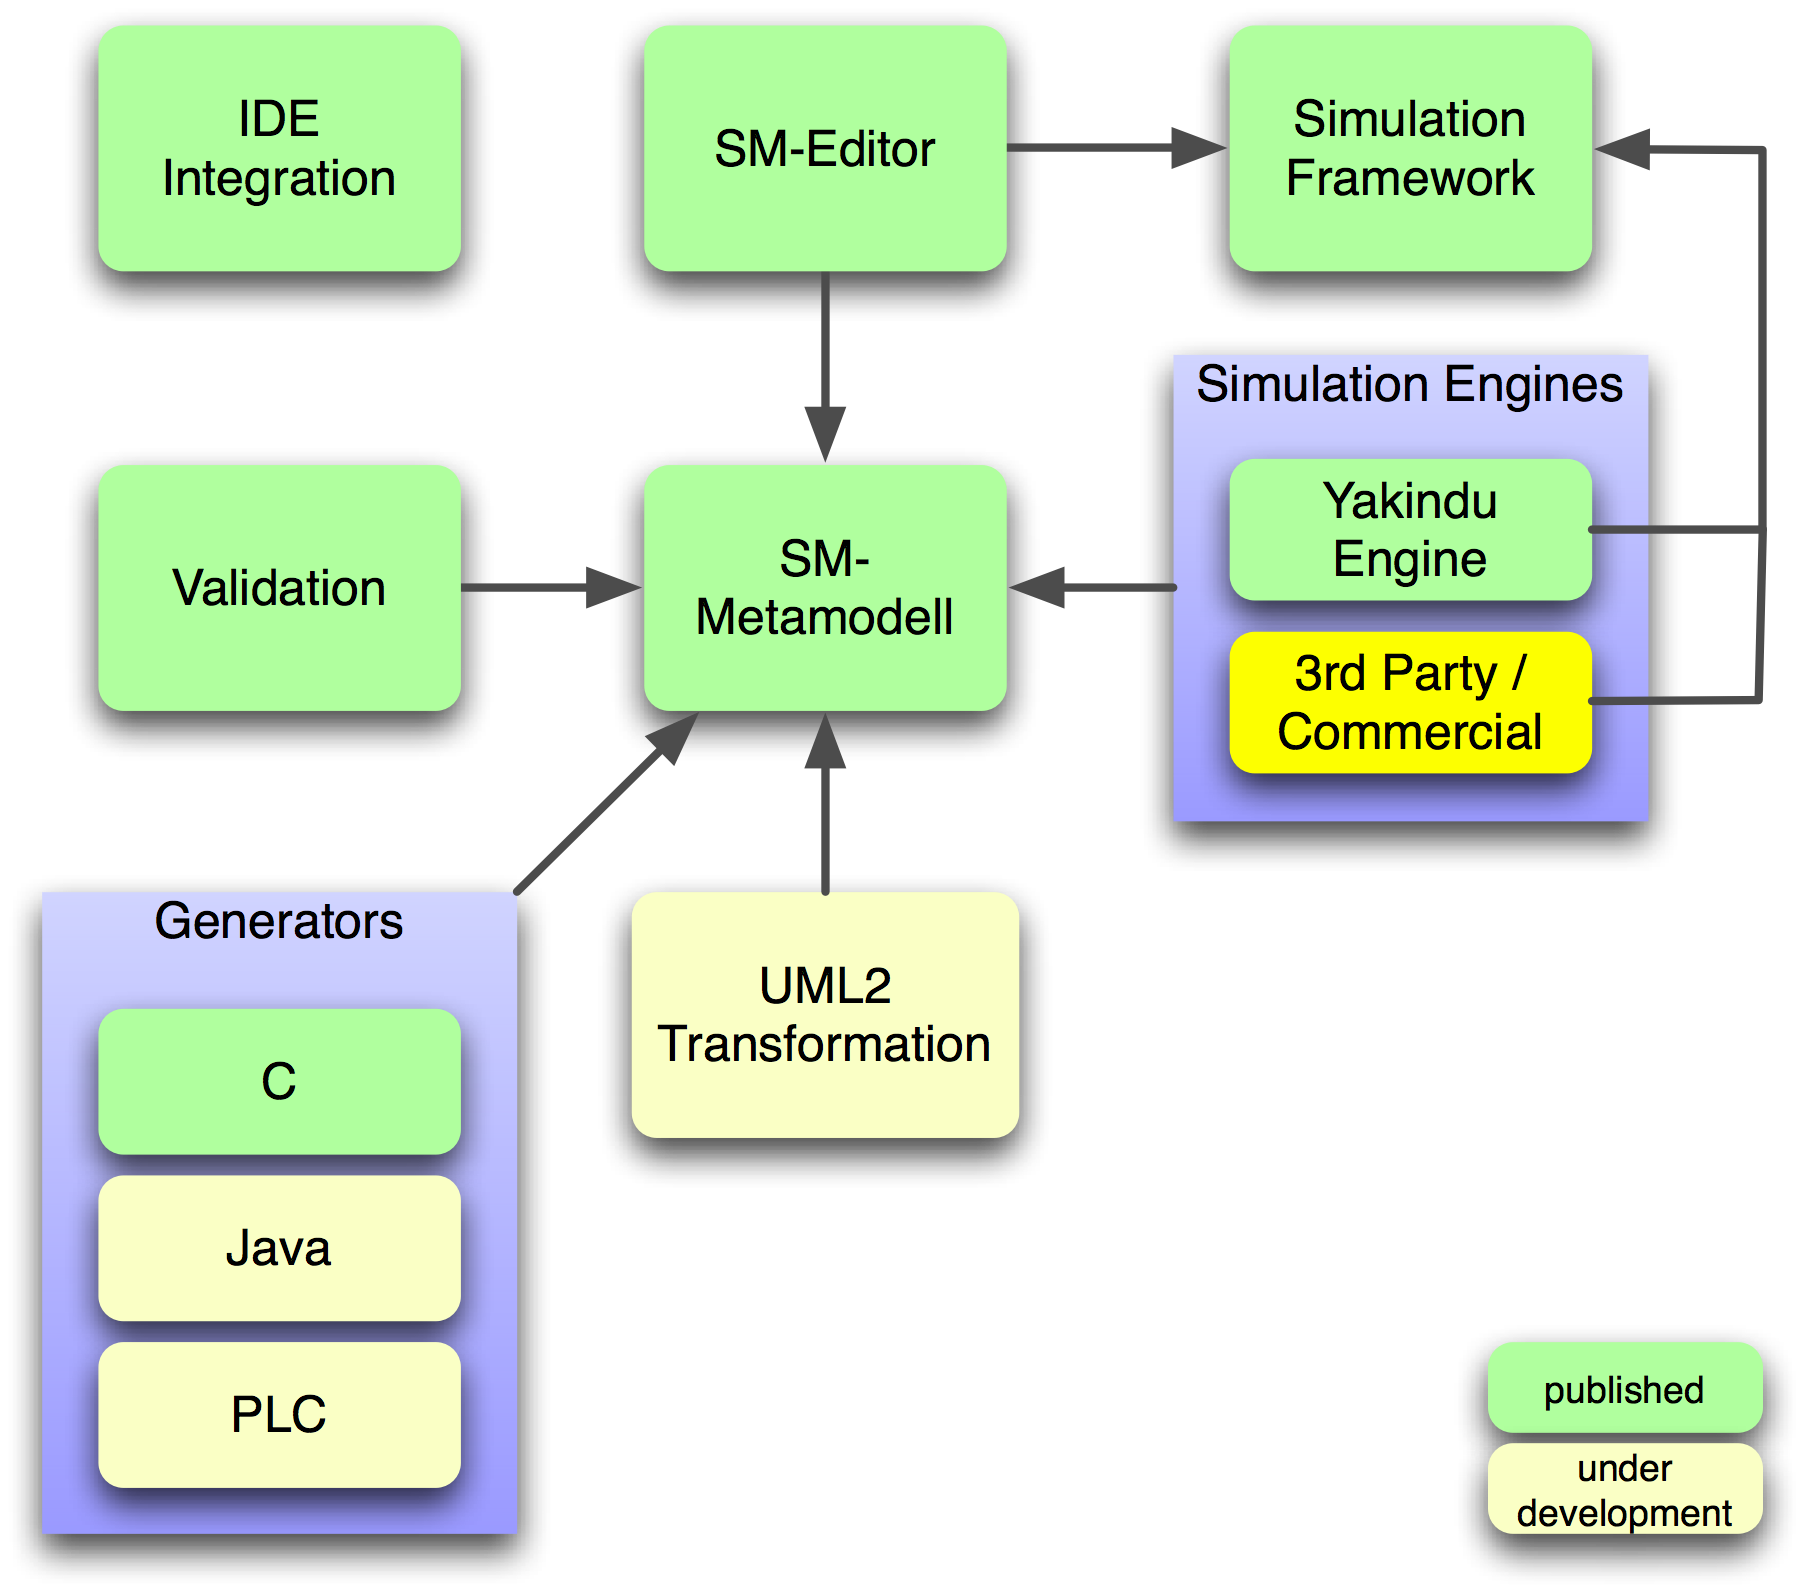
\includegraphics[width=0.7\textwidth]{Pictures/ToolArchitektur}
\caption{\label{fig:toolArchitecture}Tool architecture}
\end{figure}
\clearpage


%\input{}

%%%%% Installation Guide
\chapter{Installation}
%%%%%%%%%%%%%%%%%%%%%%%%%%%%%%%%%%%%%%%%%%%%%%%%%%%%%%%%%%%%%%%%%%%%%%%%%%%
% Copyright (c) 2010 committers of YAKINDU and others.
% All rights reserved. This program and the accompanying materials
% are made available under the terms of the Eclipse Public License v1.0
% which accompanies this distribution, and is available at
% http://www.eclipse.org/legal/epl-v10.html
%
% Contributors:
%     committers of YAKINDU - initial API and implementation
%%%%%%%%%%%%%%%%%%%%%%%%%%%%%%%%%%%%%%%%%%%%%%%%%%%%%%%%%%%%%%%%%%%%%%%%%%%
\section{Eclipse Installation}

The YAKINDU Plugin installation follows the usual eclipse installation process.

However, before you start, be sure to have the Eclipse environment (3.6/Helios)
installed. You can download eclipse distributions from the Eclipse download site.

\url{http://www.eclipse.org/downloads/}

Please be aware that there are many different distributions supporting different
features. When installing the YAKINDU features the required features will be
installed automatically if they are not already installed. You can also download
the itemis oAW distribution that already contains several required plugins.

%\url{http://oaw.itemis.com/openarchitectureware/language=en/2837/downloads}
\url{http://oaw.itemis.com/downloads/}

The YAKINDU statechart tools require several Eclipse plugins:

\begin{itemize}
\item EMF
\item GEF
\item GMF
\item Xtend
\item Xpand
\item Xtext
\item MWE
\item and some others\dots
\end{itemize}

Additionally you may want to install additional features like the CDT (C/C++
Development Tools) or the JDT (Java Development Tools). You can install them with
the same mechanism as described in the next section.

\section{Installing the YAKINDU-Plugins}

To install the YAKINDU plugins, open the \textbf{Software Updates and Add-Ons}
dialog which can be found at Help$\rightarrow$ \textbf{Install New Software...} (like
\ref{fig:updatesMenu}). \begin{figure}[ht] \center
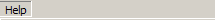
\includegraphics[width=0.3\textwidth]{Pictures/helpMenu}\\
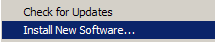
\includegraphics[width=0.3\textwidth]{Pictures/softwareUpdates}
\caption{\label{fig:updatesMenu}Menu to select software updates} 
\end{figure}
In the window press the \textbf{Add ...} button and enter the update site URL
\url{http://updates.yakindu.com/helios/release/}
into the \textit{Location} area (see Figure \ref{fig:updateSite}). After
accepting the new URL the update site will be queried.

\begin{figure}[ht]
\center
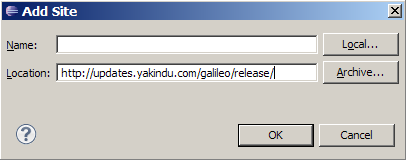
\includegraphics[width=0.7\textwidth]{./Pictures/updateSite}
\caption{\label{fig:updateSite}Update site for YAKINDU} 
\end{figure}

If everything is correct, you will find a new entry \textit{YAKINDU Update Site}
in the list in the \textit{Available Software} tab. Before continue it is
neccessary to acitvate update sites for MWE, Xpand and Xtext. This is
done by clicking on \textbf{Manage Sites\dots} and selecting the Helios update site.
\begin{figure}[ht]
\center 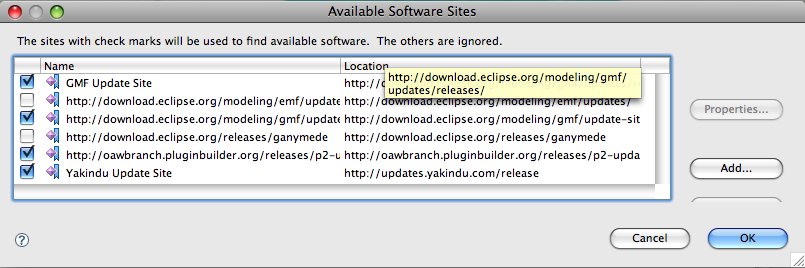
\includegraphics[width=0.5\textwidth]{./Pictures/manageSites}
\caption{\label{fig:manageSites}Select update site for dependency resolving} 
\end{figure}

For quick start check the Feature \textit{YAKINDU Feature}, \textit{MWE SDK}, 
\textit{Xpand SDK} and \textit{Xtext SDK} below the tree of
\textit{YAKINDU Update Site} and \textit{Helios Update Site}. After select the 
Features press the \textbf{Install} button. For  the
first installation many dependencies are downloaded and you have to wait some
minutes.

\begin{figure}[ht]
\center
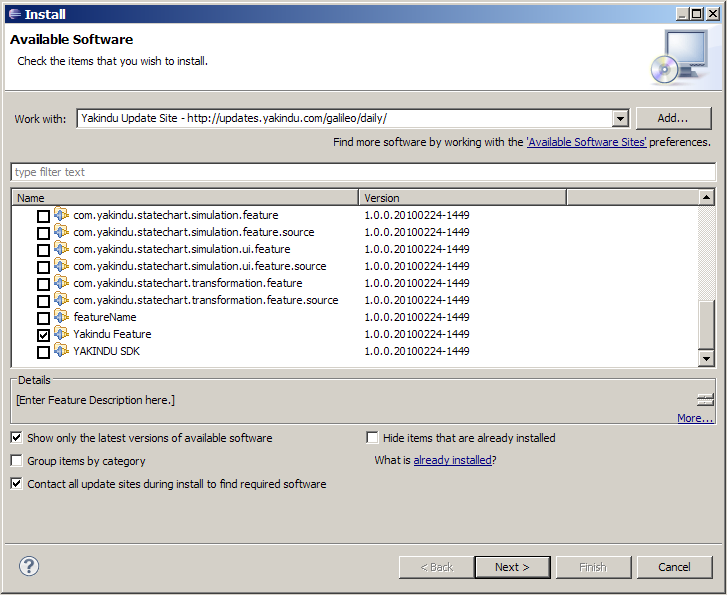
\includegraphics[width=0.45\textwidth]{./Pictures/updateSelected}
\caption{\label{fig:Update}Software Updates and Add-Ons Install Dialog} 
\end{figure}

In the next steps you have to confirm the selected Features (see Figure
\ref{fig:confirmFeatures}) and accept the License after reading it. Confirm the Security
Warning by clicking the "Ok" button. The next
steps are automatic and are finished by an information box from eclipse, asking
you to restart. Answer with \textit{Yes}, because YAKINDU becomes active after
restart.

\begin{figure}[ht] \center
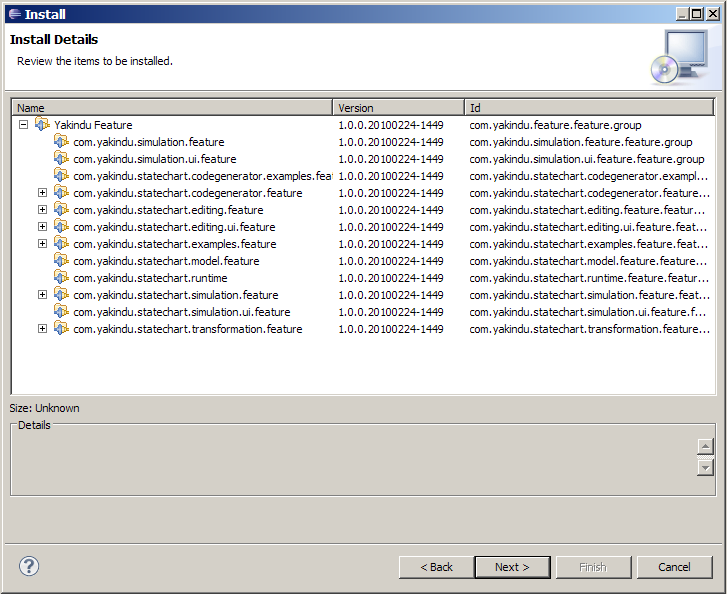
\includegraphics[width=0.45\textwidth]{./Pictures/featureConfirm}
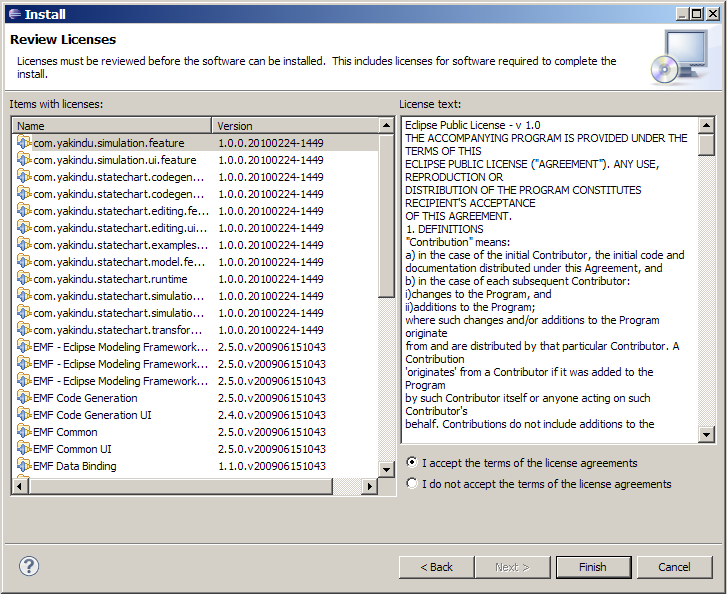
\includegraphics[width=0.45\textwidth]{./Pictures/licences}
\caption{\label{fig:confirmFeatures}Confirm selected features and the license} 
\end{figure}

After a few seconds, your installation is ready to run the quick start example
presented in the next section. Before we continue it is a good idea to change the
perspective to YAKINDU. With this perspective all main tools from the
YAKINDU-Toolchain are directly accessible. Although it's also possible to add
some of this views to your favourite perspective and edit statecharts in parallel
to your all day work.

It is highly recommended that you update your plugins after installation via 
\textit{Help}$\rightarrow$ \textit{Check for Updates}. So you get the actual
version of the YAKINDU-Statechart Tools.

\newpage
\section{Installing from Zip}

The YAKINDU-Web Site also provides a zip file with all plugins for download. The
dependencies to GMF must be satisfied manually. The update sites for eclipse 
are the following and the required features are mostly the sdks of the plugins 
mentioned before:

\begin{itemize}
\item EMF Update Site: \url{http://download.eclipse.org/modeling/emf/updates/}
\item GMF Update Site: \url{http://download.eclipse.org/modeling/gmf/updates/releases/}
\item Helios Update Site: http://download.eclipse.org/releases/helios
\item Xtext \url{http://xtext.itemis.com/downloads/}
\item and some others\dots
\end{itemize}



%%%%% Modelling and Simulation Tutorial
\chapter{Statechart Modelling and Simulation}
%%%%%%%%%%%%%%%%%%%%%%%%%%%%%%%%%%%%%%%%%%%%%%%%%%%%%%%%%%%%%%%%%%%%%%%%%%%
% Copyright (c) 2010 committers of YAKINDU and others.
% All rights reserved. This program and the accompanying materials
% are made available under the terms of the Eclipse Public License v1.0
% which accompanies this distribution, and is available at
% http://www.eclipse.org/legal/epl-v10.html
%
% Contributors:
%     committers of YAKINDU - initial API and implementation
%%%%%%%%%%%%%%%%%%%%%%%%%%%%%%%%%%%%%%%%%%%%%%%%%%%%%%%%%%%%%%%%%%%%%%%%%%%

Now follows a quick introduction into the YAKINDU tools and the usage. For a
deeper understanding you can read the later chapters.
\section{The YAKINDU Perspective}
\begin{floatingfigure}[r]{0.3\textwidth}
  \centering
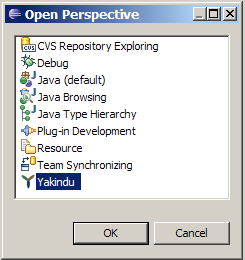
\includegraphics[width=0.3\textwidth]{./Pictures/yakinduPerspectiveSelection}
\caption{\label{fig:perspectiveSelection}Selecting the YAKINDU Perspective} 
\end{floatingfigure}
The YAKINDU tools comes with an easy perspective for quick starting and using it.
The perspective can be activate by clicking on \textbf{Window} $\rightarrow$
\textbf{Open Perspective} $\rightarrow$ \textbf{Other} and selecting the YAKINDU
perspective (Figure \ref{fig:perspectiveSelection}). After activation the screen
looks like figure \ref{fig:perspective}.

In the middle the main view on screen is the editor. It is still empty, but you
will use it most often. On the left is also a default eclipse view, the project
explorer. You will need it for the next step. The other views will be described
later, when they are needed.

\begin{figure}[ht]
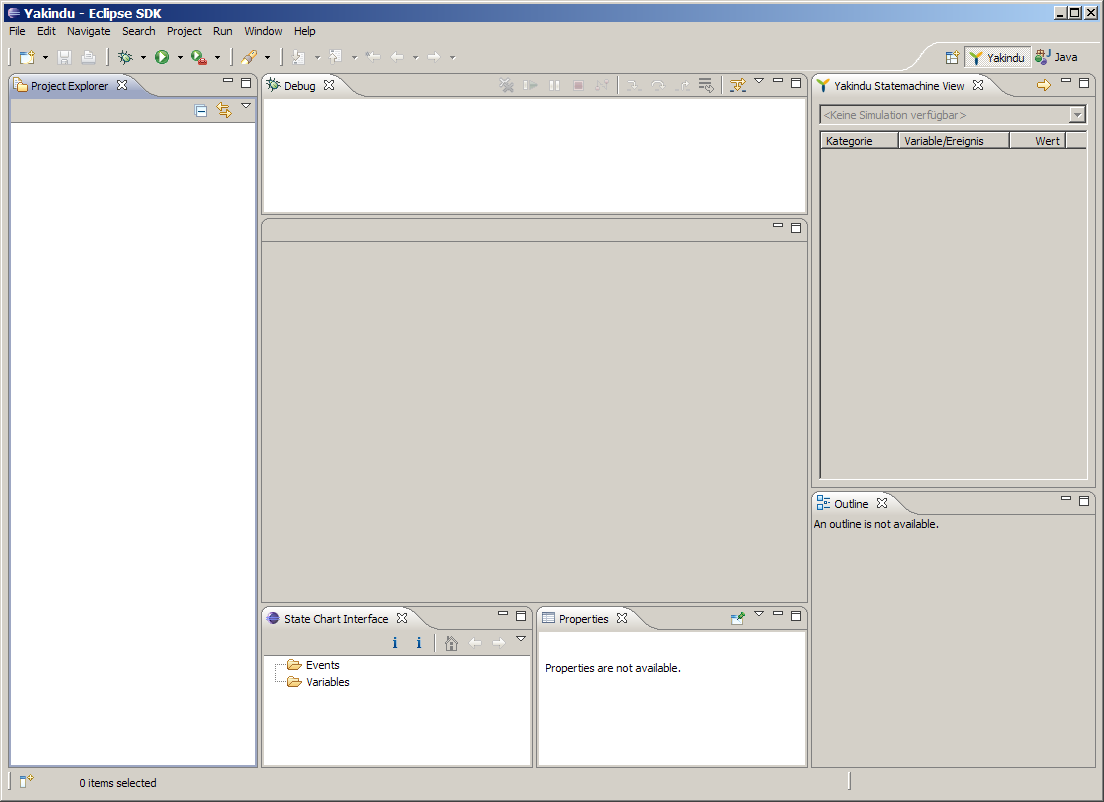
\includegraphics[width=0.5\textwidth]{./Pictures/perspective}
\caption{\label{fig:perspective}The YAKINDU Perspective} 
\end{figure}



\pagebreak
\section{Example Step by Step}

When YAKINDU is properly installed, we can start a small example project. This
example project gives an idea of how powerful the YAKINDU tool-chain is. It
contains a visual editor, a semantic and logic verification check, a simulator
unit and a number of code generators.

To present the visual editor, the check mechanism and the simulator of the
YAKINDU tool-chain, an example was chosen, that is simple enough to give an
impression of the usage but is not to far-fetched.

\subsection{Example State Machine}

The idea is to have a state machine, that represents a staircase lighting. This
staircase lighting is started with a key-press and stops after 30 seconds.

The state machine itself consists of two states: ,,Lights On'' and ,,Lights
Off''. The standard state within the state machine is ,,Lights Off'' and is
entered from start-up (the so called initial state). When an occupant enters the
staircase and presses the lighting button, a ,,keypress'' event is generated
which starts the transition to the ,,Lights On'' state.

On entering the state ,,Lights On'', the staircase lighting is turned on. When
the retention period has expired (after 30 seconds), the ,,Lights On'' state is
left with a transition to the state ,,Lights Off'' and the lighting is turned off
again.

\subsection{Creating a new Project}

When everything is set up, your Eclipse editor should look similar to this:

\begin{figure}[ht]
\centering
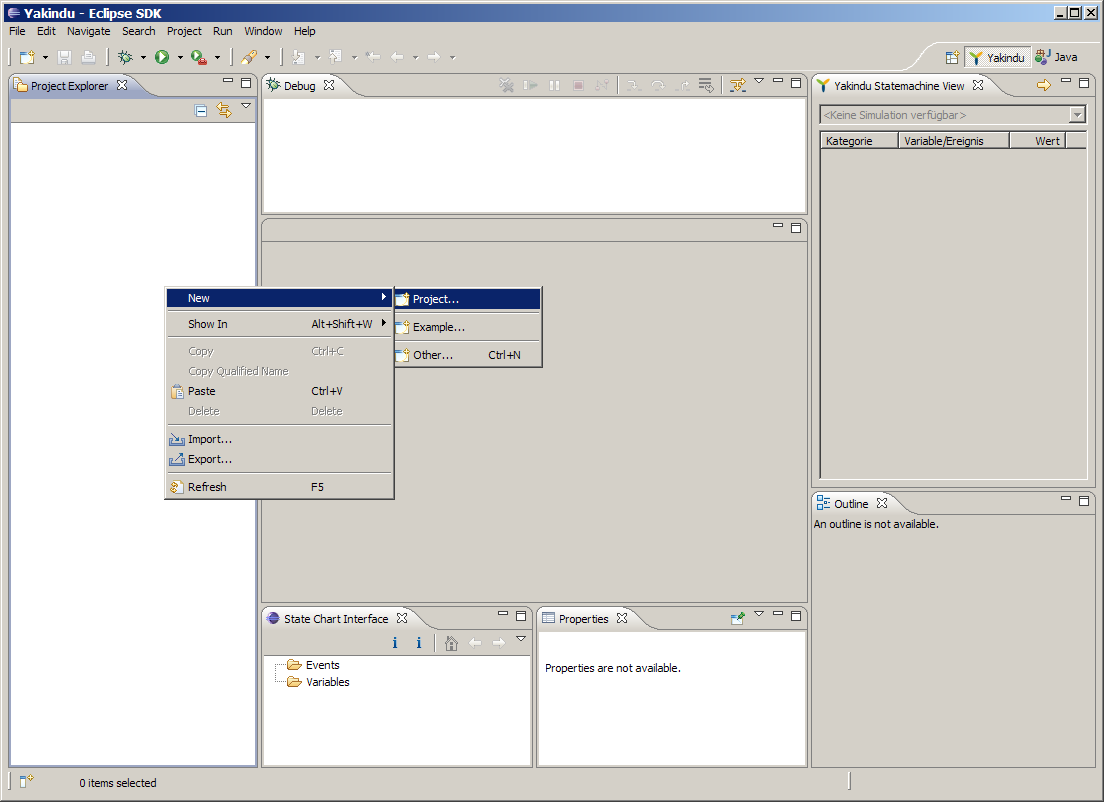
\includegraphics[width=0.8\textwidth]{./Pictures/NewProject}
\caption{\label{fig:NewProject}Creation of a new project} 
\end{figure}
\newpage
\begin{figure}[h!]
\centering
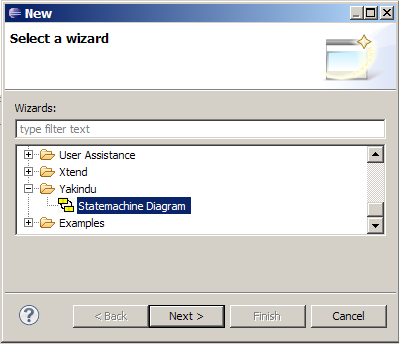
\includegraphics[width=0.5\textwidth]{./Pictures/Wizard}
\caption{\label{fig:wizard}Wizard to create a new State Machine}
\end{figure}

To start a new project, open the menu (\textbf{File$\rightarrow$ New$\rightarrow$
Project}) and create a new Java Project. In our example, the project is called
,,\textit{Example}''.  However, this procedure only creates a default Java
project. For simplicity you should deny the question for changing to Java
perspective, because we won't use anything from Java. \newpage
\begin{floatingfigure}[r]{0.3\textwidth}
\centering
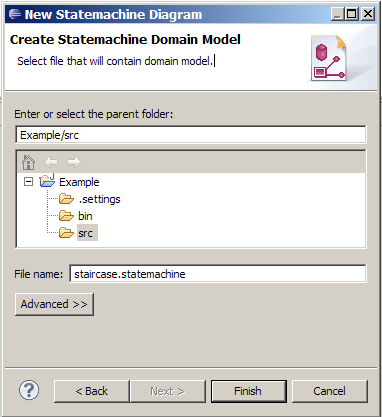
\includegraphics[width=0.3\textwidth]{./Pictures/Wizard2}
\caption{\label{fig:wizard2}Wizard to create a new state machine domain model}
\end{floatingfigure}
To create a \textbf{state machine model} to this environment, right-click the
\textbf{src} directory icon and open the select wizard at
\textbf{New$\rightarrow$ Other}. Here you have to select \textbf{state machine
Diagram} from the \textbf{YAKINDU} folder as shown on figure \ref{fig:wizard}.

Figure \ref{fig:wizard2} displays the \textit{New Statemachine Diagram} window,
in which the name of the state machine model is set. In our example, the name is
changed from \textbf{default.statemachine} to staircase.statemachine.

The wizard has then created two sources: the \textbf{staircase.state\-machine}
and the \textbf{staircase. state\-machine\_\-diagram}. The state machine itself
is represented as an XML-file in \textbf{staircase. state\-machine} and the
visual representation of the state machine can be found in the
\textbf{staircase.state\-machine\_\-diagram} file.


Now you should have a new visual editors view to create a state machine as shown
in figure \ref{fig:YEditor}. Here you have all elements to create a state machine
from bottom up in the elements menu. The elements that are important for our
small project are 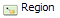
\includegraphics[height=12pt]{./Pictures/Region},

\includegraphics[height=12pt]{./Pictures/State},
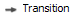
\includegraphics[height=12pt]{./Pictures/Transition} and

\includegraphics[height=12pt]{./Pictures/InitialState}.

\begin{figure}[ht]
\center
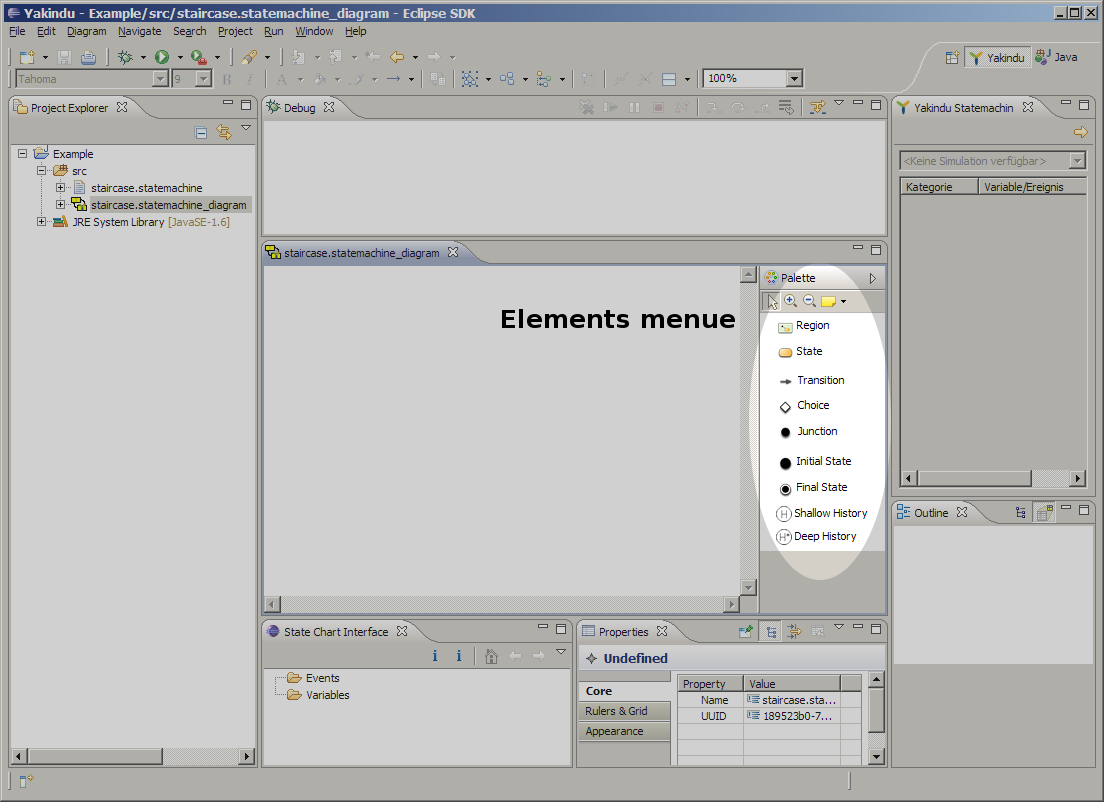
\includegraphics[width=\textwidth]{./Pictures/YakinduEditor_1}
\caption{\label{fig:YEditor}YAKINDU State Machine editor}
\end{figure}
 
\subsection{Defining a State Machine}

%Creating a state machine is quite easy:

To start with the visual editor you firstly need a region, in which the states of
the state machine reside. Therefore you need to click the
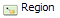
\includegraphics[height=12pt]{./Pictures/Region} icon and draw a region on the
empty plain. When you have placed the last corner of the region and you release
the mouse button, a new region in light green appears. At the properties area,
the priority of this region is highlighted and should be set to a value. As we do
not have any concurrent regions in this example, the priority is not important
and could be set to any valid integer value (10 in our example). If you use more
than one region, the priority specifies the processing order in which the states
actions and the states transitions are processed.

% ToDo (for further information please refer to section \ref{sec:Regions}).

To set the priority of the region afterwards, you can open the properties view.
If you cannot find it in your eclipse perspective, you can open it by clicking
\textbf{Window$\rightarrow$ Show View$\rightarrow$ Others} and in that menu:
\textbf{General$\rightarrow$ Properties}.

Now as you have created a region, you need a starting point of your state
machine. This starting point is called \textbf{initial state} and can also be
found as an icon (
\includegraphics[height=12pt]{./Pictures/InitialState}) in the
elements menu. As explained at the beginning of this chapter, the two states
\textbf{LightOn} and \textbf{LightOff} should be installed within the state
machine region.

To create a state, you have to select the
(
\includegraphics[height=12pt]{./Pictures/State}) element and then open the area
within the region plain. When the state outline is created, the first line within
the properties area is highlighted and needs to be filled by the name of this
state (e.g. LightOff). The name of a state has to be unique within a region.

\begin{figure}[ht] \center
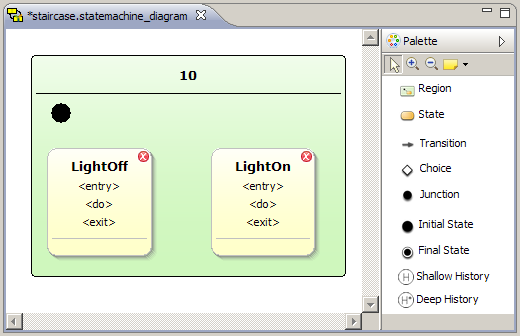
\includegraphics[width=0.7\textwidth]{./Pictures/StateCreation_1}
\caption{\label{fig:StateCreation}Creation of the \textbf{Initial}, 
\textbf{LightOff} and \textbf{LightOn} state}
\end{figure}
% \clearpage

After the creation and naming of the states, the actions ($<entry>$, $<do>$,
$<exit>$) should be created. In our case, the only action that should be
performed is switching the light on or off. The status of the light is
represented by a variable that could hold one of the two values 1 or 0. This
variable needs to be created in the \textbf{State Chart Interface}. Within this
view, you can right-click on \textbf{Variables}, where you get a new window to
specify the variable that should be created (refer figure
\ref{fig:CreateVariable}). Here you add the variable name (\textit{Light}), the
port, the IO-type and the data type. In our example all other information except
for the variable name do not have to be changed.

\begin{floatingfigure}[r]{0.4\textwidth}
\includegraphics[width=0.4\textwidth]{./Pictures/CreateVariable}
\caption{\label{fig:CreateVariable}Creating a variable in the \textit{State Chart Interface}}
\end{floatingfigure}

%\begin{figure}[ht]
%\center
%\includegraphics[width=0.3\textwidth]{CreateVariable}
% \caption{\label{fig:CreateVariable}Creating a variable in the \textit{Data
% Element Explorer}} \end{figure}

Then you add the action \texttt{Light=0;} into the $<entry>$ line within the
states properties area (either within the Diagram or within the
\textbf{Properties} view). This definition creates a new action, that is
performed whenever the state \textbf{Light\-Off} is entered. So when the
unconditioned state transition from the \textbf{initial state} to the
\textbf{LightOff} state is performed, the internal variable \textit{Light} is set
to zero. The same takes place, when the state \textit{LightOff} is entered
through a transition from any other state.

The state \textbf{LightOn} is created in the same way, except that the action is
set to \texttt{Light=1;}.

To create a transition between the \textbf{Initial State} and the
\textbf{LightOff} state, you choose the
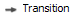
\includegraphics[height=12pt]{./Pictures/Transition} element and connect the
\textbf{Initial State} and the \textbf{LightOff} state. Every transition claims
an \textbf{expression}, when this transition should be executed.

An expression can consist of one or more \textit{triggers}, \textit{guard
operations} and \textit{actions}, which can also be mixed. Additionally a
transition must have a priority, to define the order, in which the expressions of
different, concurrent transitions are processed.
% ToDo To learn more about transition expressions, please read section
% \ref{sec:Transitions}.

In our example, the transition between the \textbf{Initial state} and the
\textbf{LightOff} state do not need any expression, as this transition has no
condition. When the expression area of a transition is left blank, the expression
is represented by an asterisk (*).

The transition between \textbf{LightOff} and \textbf{LightOn} is performed, if
the trigger \textit{keypress} was received. Therefore a new event has to be
implemented in the \textit{State Chart Interface} (refer also to figure
\ref{fig:CreateVariable}). Here you add an event that can be used as a trigger
within a transition expression. Implementing a trigger with a transition needs
only the trigger name as the expression string (\textit{keypress}).

To specify the transition from \textbf{LightOn} to \textbf{LightOff} after 30
seconds, you use the keyword $after(<duration>s)$ within the transition
expression string. The \textit{after()} expression switches to the target state
when the specified time has been expired.

So in the end your state machine looks like in figure
\ref{fig:statemachineFinish}.

\begin{figure}[ht]
\center
\includegraphics[width=0.7\textwidth]{./Pictures/statemachineFinish_1}
\caption{\label{fig:statemachineFinish}Complete State Machine (State Machine Diagram Editor)}
\end{figure}

\newpage
\subsection{Checking the State Machine}
The state chart is very common and it is possible to model things, which doesn't
make sense for your target platform or you want to have some special naming
conventions. We will check now, that every name of a state is at least eight
character long. But first we have to prepare our Project for code completion
within checks. Later on we can add a new check file and enter the checks.

\subsection{Project type and dependencies}
For this steps it is neccessary, that the model is inside an Java project. If
it's not yet, you can create a new project beside the first, copy the model and
change the target directories (see chapters \ref{sec:CCodeGenerator} and
\ref{sec:JavaCodeGenerator})  for generated files, so they point to the first.

\begin{figure}[ht]
\center
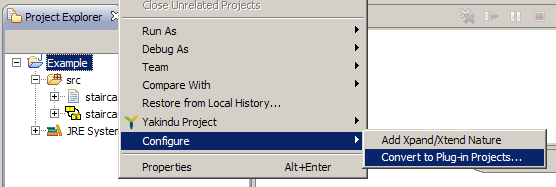
\includegraphics[width=0.7\textwidth]{./Pictures/switch_to_pde_project}
\caption{\label{fig:switchToPdeProject}Add plugin development nature to your java project}
\end{figure}
We will add the plugin development nature from eclipse to the project by
selecting the project, click with the right button and select \textbf{Configure}
$\rightarrow$ \textbf{Convert Projects to Plugin Projects\dots} (Picture
\ref{fig:switchToPdeProject}). Your project is already selected in the next
window and you can press Finish to complete. As a result some new files are
created in your project. We only need the \textbf{MANIFEST.MF} inside the folder
\textbf{META-INF}. Open this file by double-click and add some dependencies (See
picture \ref{fig:manifest}). This is done by clicking on \textbf{Add} and
selecting some plugins. If you design for codegeneration the plugin
\textit{com.yakindu.statechart.codegenerator.java} or
\textit{com.yakindu\dots{}c} are the one of your choice. For platform independent
modeling you can select \textit{com.yakindu.statechart.model.expressions}.
\begin{figure}[ht] \center
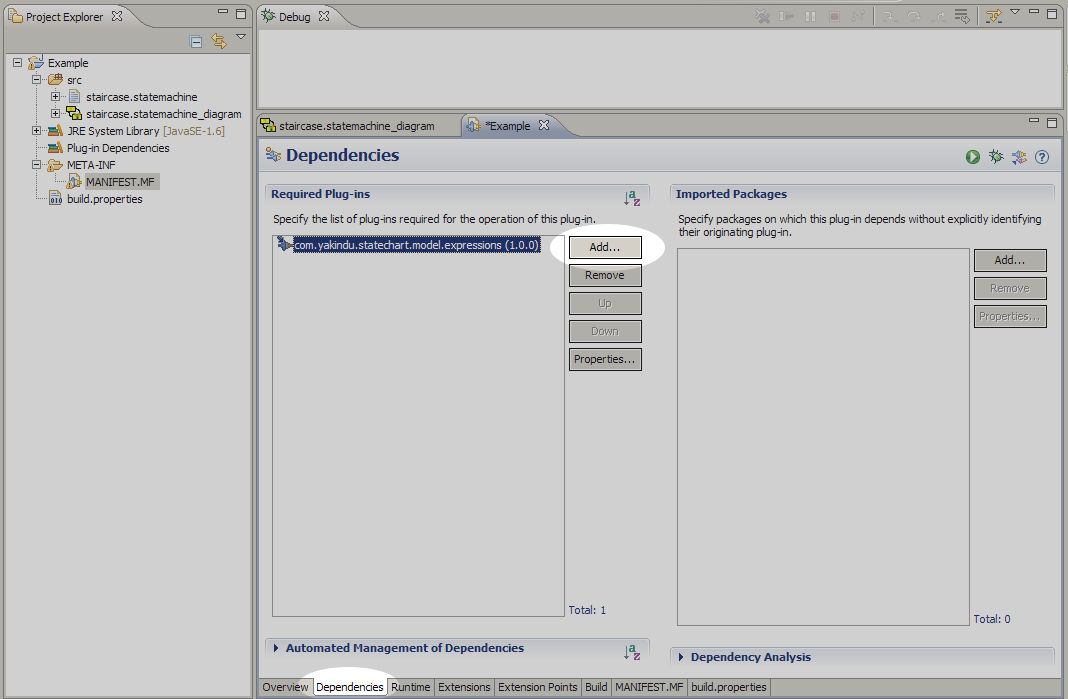
\includegraphics[width=0.7\textwidth]{./Pictures/manifest}
\caption{\label{fig:manifest}Add dependencies to your project}
\end{figure}

Now the file can be saved and closed. It will not be neccessary to edit this file
later, except you decide to use an additional codegenerator.

\subsection{Create check files}
All user defined check files reside in a folder names checks. Within this folder
all \textbf{.chk}-files are evaluated and considered for checking. The format of
check files is described in the reference of eclipse modeling project and the old
openArchitectureWare-project\footnote{http://oaw.itemis.de/openarchitectureware/662/ressourcen}.

Create a new folder in the root of your project by right-click on
\textbf{Examples}  and selecting \textbf{New}$\rightarrow$\textbf{Folder}. The
folder must be named \textit{checks} and the other options can be ignored. Simply
finish and create your check files inside this folder.

Check files are created by selecting the folder ''checks'' and choosing in the
drop-down-menu the entry \textbf{New}$\rightarrow$\textbf{Other}. In the next
window the entry \textbf{Check file} is found inside the category
\textbf{Xtend}(see Figure \ref{fig:newCheckFile}.

\begin{figure}[ht] \center
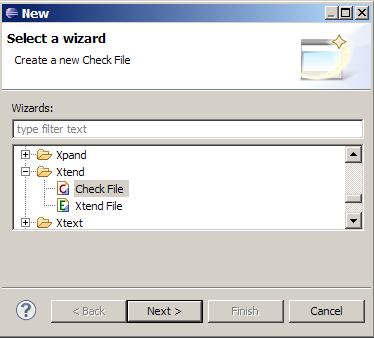
\includegraphics[width=0.7\textwidth]{./Pictures/newoAWCheckFile}
\caption{\label{fig:newCheckFile}Add a new check file to your project}
\end{figure}

\subsection{Editing check files}
The syntax of check files is described in the oAW-Reference, but the short
introduction here is enough for the first experience. If you try the code
completion (\texttt{Strg+space}) the first time in the editor, you are asked to
add the Xtend nature to your project (See figure \ref{fig:addOAWNature}). Answer
with yes, to get code completion. \begin{figure}[ht] \center
\includegraphics[width=0.7\textwidth]{./Pictures/addoAWNature}
\caption{\label{fig:addOAWNature}Add the Xtend nature to your project for code completion}
\end{figure}

Every check file starts with an \texttt{import} of the required and used models.
For the statemachine it is sufficient to add the model \texttt{statemachine}.
After this we want to add a check for a state. This is done by defining a
\texttt{context} for the model element \texttt{State} and the severity of
\texttt{WARNING} or \texttt{ERROR}. Because short names are not nice and we
spelling names we define an error with the error message ''State names must have
at least 8 characters''. After a colon the boolean expression folows. The
expression defines the default, not the error. In our case names are longer or
equals to eight characters. In figure \ref{fig:nameLengthCheck} the result of
''state.chk'' is printed.

\begin{figure}[ht] \center
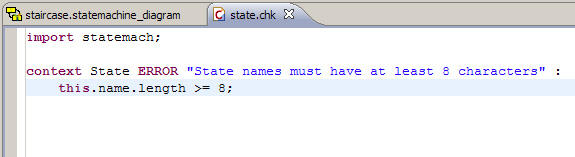
\includegraphics[width=0.7\textwidth]{./Pictures/nameLengthCheck}
\caption{\label{fig:nameLengthCheck}An example check file for names longer 
than eigth characters}
\end{figure}

After saving the file and opening the statechart again, the statechart is
validated after some seconds. As a result you can see a red cross in the upper
right corner of state LightOn. That's because we added a check, that state names
must have at least eight characters and LightOn needs only seven characters. If
you put the mouse above the red cross and wait some seconds, the error message is
shown in a small box.

\subsection{Simulating a State Machine}
\label{sec:simulatingStateMachine}
When the state machine diagram is completed, you can start a simulation session,
to check, whether your new state machine is working correctly.

To start a simulation you have to create a new \textit{run} configuration, as
shown in figure \ref{fig:SimulationStart}. Choose the entry \textbf{Run
Configuration ...} to open the configuration dialog.

\begin{figure}[ht] \center
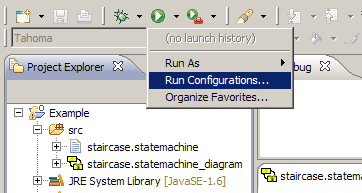
\includegraphics[width=0.4\textwidth]{./Pictures/startSimulation_1}
\caption{\label{fig:SimulationStart}Starting the Simulation creation dialog}
\end{figure}

In this dialog you add a new \textbf{YAKINDU Simulation} called \textit{Example}
by clicking the 'New' button in the upper left corner. Then the configuration
dialog is presented. After choose your \textit{Example} project and the staircase
state machine as your model file the dialog looks like figure
\ref{fig:SimulationCreation}. As your simulation engine, please choose
\textit{YAKINDU Statechart Simulator}.

\begin{figure}[ht]
\center 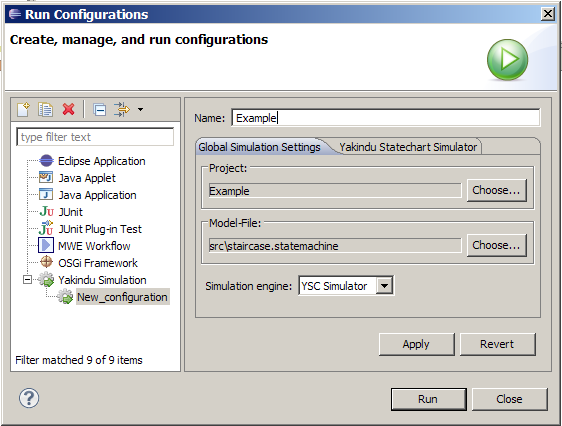
\includegraphics[width=0.7\textwidth]{./Pictures/SimulationCreation}
\caption{\label{fig:SimulationCreation}Dialog to create a new simulation environment}
\end{figure}

When you click the \textbf{Run} button in the lower right corner, you start the
simulation. To rerun the simulation later, you find an entry \textit{Example} in
your \textbf{Run} configuration.

\begin{figure}[ht] \center
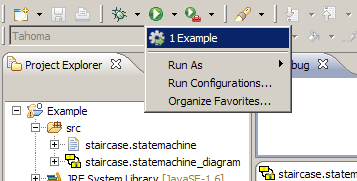
\includegraphics[width=0.4\textwidth]{./Pictures/runLater_1}
\caption{\label{fig:runLater}Restart a simulation in the menu}
\end{figure}

On Simulation start-up make sure, that the debug view is open (refer figure
\ref{fig:runningSim_1}). In this view, the simulation process can be started,
stopped and paused. Additionally the simulation can be used in single step modus.
To activate the single step modus, the simulation must be in the pause position.
When a single step should be performed, the single step button can be pressed.
The advantage in this modus is, that you can set the input parameter according to
your simulation scenario and perform the next step, when you are done with that.
To be able to change the events and variables, you must have started the
simulation explicit by a click to the run button in the debug view, or by
clicking on the single step button.

To be able to interact with the simulation by the input values, open the
\textbf{YAKINDU Statemachine View}. This view can be found in the main menu under
\textbf{Window}$\rightarrow$ \textbf{Show View}$\rightarrow$ \textbf{Other...}.
In the appearing menu choose \textbf{YAKINDU Statemachine}.

\begin{figure}[ht] \center
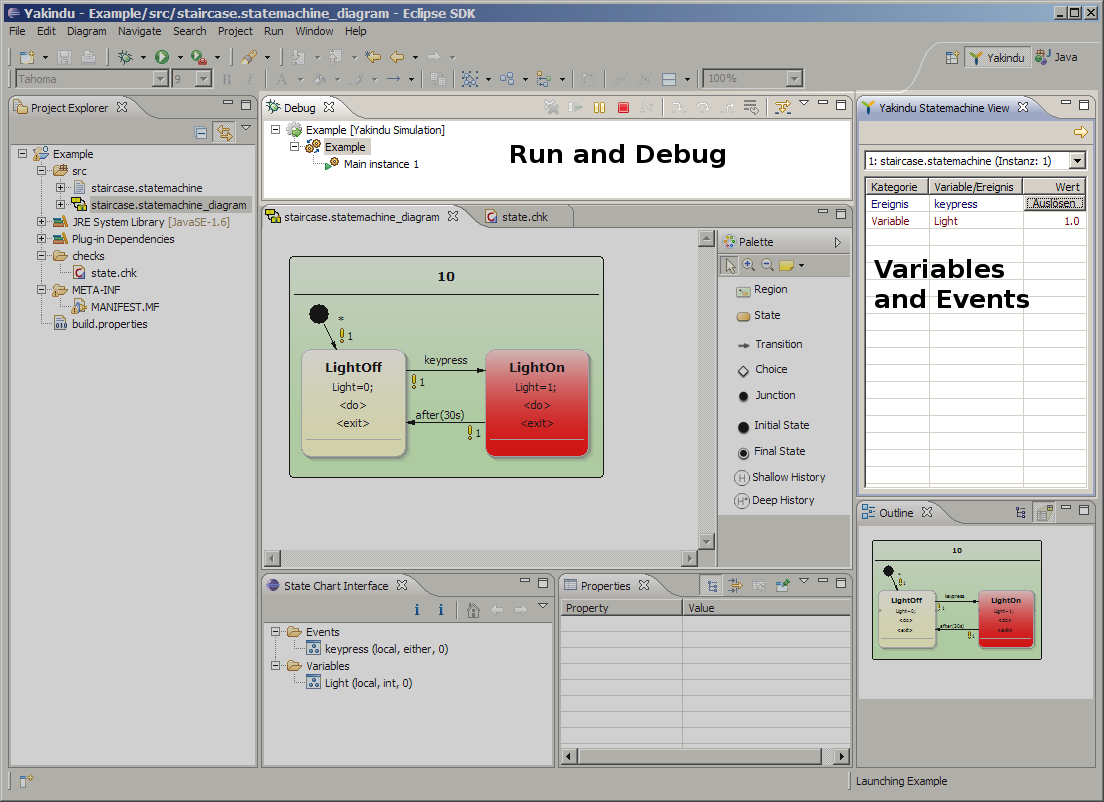
\includegraphics[width=0.7\textwidth]{./Pictures/runningSim_1_1}
\caption{\label{fig:runningSim_1}Running a simulation}
\end{figure}
 
% \begin{floatingfigure}[r]{0.3\textwidth}
% 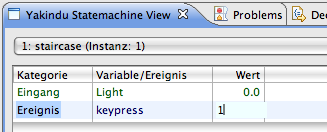
\includegraphics[width=0.3\textwidth]{./Pictures/runningSim_2}
% \caption{\label{fig:runningSim_2}Change trigger value during simulation}
% \end{floatingfigure}

In our example project, the state machine starts with a transition from the
initial state to the \textit{LightOff} state. This state transition is visualized
by a red arrow. During a simulation an active state is highlighted in red.

\begin{figure}[ht] \center
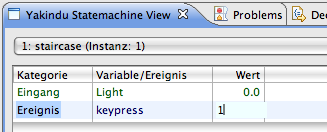
\includegraphics[width=0.4\textwidth]{./Pictures/runningSim_2}
\caption{\label{fig:runningSim_2}Change trigger value during simulation}
\end{figure}

After the active state has changed into \textit{LightOff}, this state can only be
left by a transition to \textit{LightOn}. The condition expression is set to the
trigger \textit{keypress}. This trigger can be created in the YAKINDU
Statemachine View during simulation time.  To simulate a keypress, just click the
''fire'' button near the \textit{keypress} event in Statemachine view. In this
case, the value changes and the transition is followed. After the transition has
been performed, the trigger for the transition is reset.

\begin{figure}[ht] \center
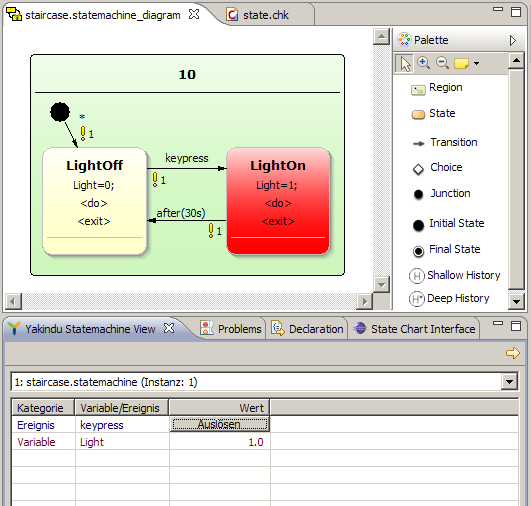
\includegraphics[width=0.7\textwidth]{./Pictures/runningSim_3}
\caption{\label{fig:runningSim_3}Trigger \textit{keypress} was activated and
the state \textit{LightOn} has been reached}
\end{figure}

The same procedure is valid to set a value of a variable. The difference between
a variable and a trigger is that a trigger value is reset to zero as soon as the
trigger has taken effect, e.g. a transition was successful. A variable value is
only changed when it is actively changed by the user or an action e.g. in
$<entry>$ $<do>$ or $<exit>$.


\pagebreak
\section{Using Example Projects}
\label{sec:exampleProjects} 

Some example projects are included in the YAKINDU release. They can be installed
by creating the \textbf{Statemachine example project}. This is done by selecting
\textbf{File} $\rightarrow$ \textbf{New} $\rightarrow$ \textbf{Statemachine
example project}. This Wizard (see Figure \ref{fig:exampleWizard}) creates after
all three new projects in your workspace, called ''Safe'', ''StaircaseLighting''
and ''TrafficLight''. You can read a short description of them, if you select
one. After you click finish the new projects are listed in your project explorer.

\begin{figure}[ht] \center
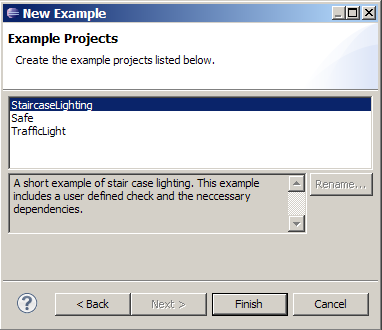
\includegraphics[width=0.6\textwidth]{./Pictures/examplesWizard}
\caption{\label{fig:exampleWizard}The state machine examples} 
\end{figure}

Taking a deeper look at the files inside the examples (Figure
\ref{fig:easyExamples}), the two projects Safe and StaircaseLighting contain only
two files. The \textit{.statemachine} file contains the model of your state
machine, and the \textit{.statemachine\underline{ }diagram} file is for
modelling. Both files are necessary to simulate and visualize the simulation. If
no visualization is needed, the model themself is enough. How to simulate is
described in section \ref{sec:simulatingStateMachine}.

The files inside the third project, the TrafficLight model, includes also model
files inside the model directory, but also an workflow under workflow and an
complex simulation environment for practical usage with a microcontroller. This
set up and handling is described in the next section \ref{sec:CCodeGenerator}

\begin{figure}[htbp] \center
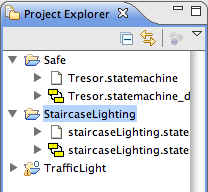
\includegraphics[width=0.3\textwidth]{./Pictures/easyExamples}
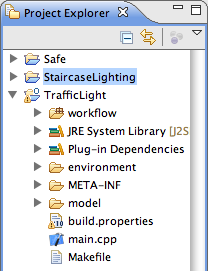
\includegraphics[width=0.3\textwidth]{./Pictures/complexExample}
\caption{\label{fig:easyExamples}Example projects and files inside} 
\end{figure}

Now we will start with a short hands-on example to demonstrate how development is
done and what especially the elements and views are for. This step is orthogonal
to-the-ready to use examples in this section.

\clearpage


%%%%% C Generator Docs
\chapter{C-Code Generator}
\label{sec:CCodeGenerator}
%%%%%%%%%%%%%%%%%%%%%%%%%%%%%%%%%%%%%%%%%%%%%%%%%%%%%%%%%%%%%%%%%%%%%%%%%%%
% Copyright (c) 2010 committers of YAKINDU and others.
% All rights reserved. This program and the accompanying materials
% are made available under the terms of the Eclipse Public License v1.0
% which accompanies this distribution, and is available at
% http://www.eclipse.org/legal/epl-v10.html
%
% Contributors:
%     committers of YAKINDU - initial API and implementation
%%%%%%%%%%%%%%%%%%%%%%%%%%%%%%%%%%%%%%%%%%%%%%%%%%%%%%%%%%%%%%%%%%%%%%%%%%%
\section{Introduction}
In our previous examples we created a YAKINDU state chart with the YAKINDU
Statechart Editor. However, it is also possible to import an existing UML2
state machine or create one with your favourite UML2 tool (You may also use
the UML2 Editor which ships with the eclipse modelling distribution). The tool
of your choice must support "EMF UML2". In our examples we are going to use
the UML2-Toools available in Galileo.

If you want to use an UML2 modelling tool instead of the YAKINDU Statechart
Editor or you have an existing UML2 state machine, you need to consider that
the YAKINDU state charts are somehow different from the UML2 state machines.
To fill this gap you have to extend your UML2 state machine (In future
releases another approach may also be available).

%or, if this is not anoption, you can create extensions for the transformation.

\section{UML2 model}
As for the code genenerators, an example project for transformation of UML2
state machines to YAKINDU state charts is also available. You can open the
examples (see Figure \ref{fig:uml2tools}) and compare them with the generated
YAKINDU state charts. \begin{figure}[ht]
\center
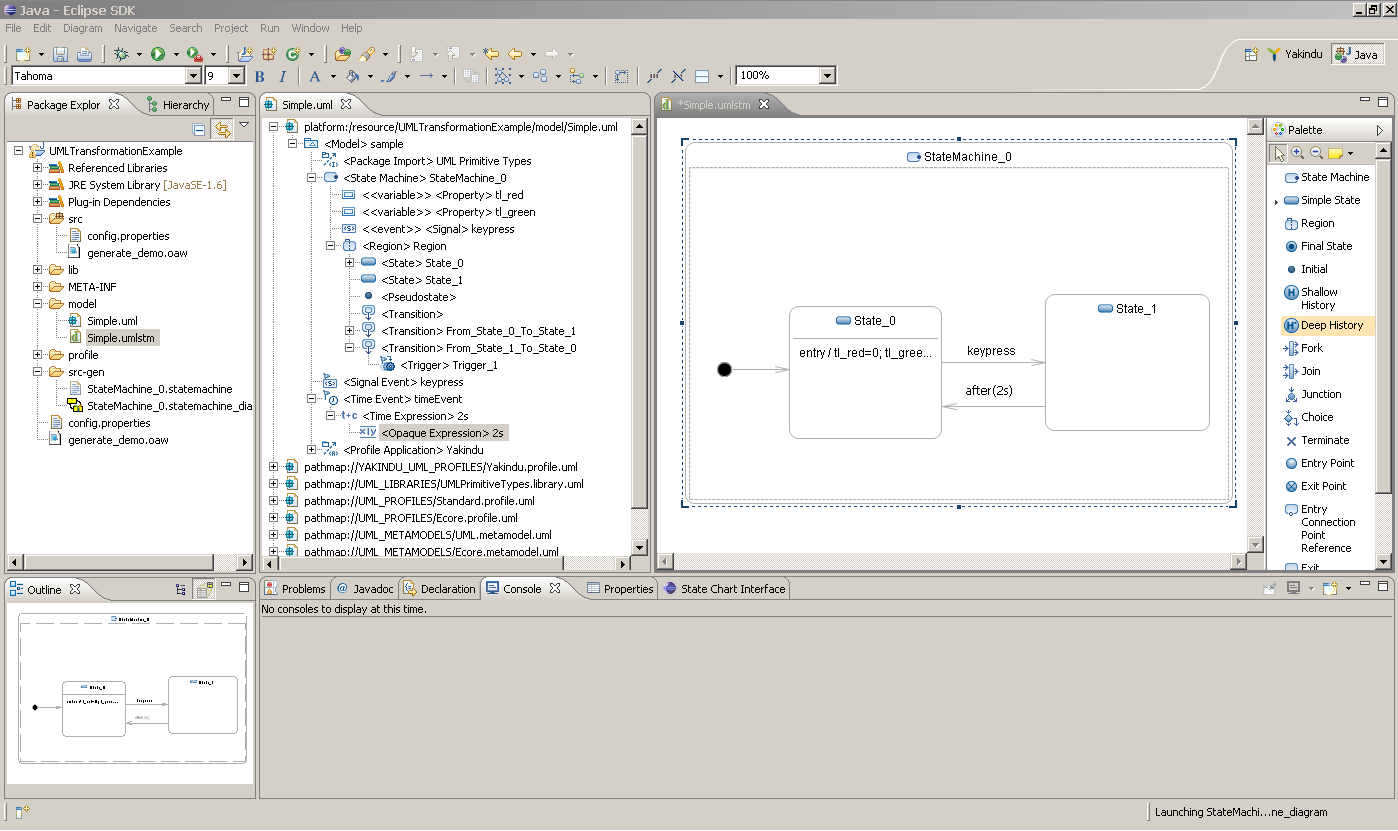
\includegraphics[width=1\textwidth]{Pictures/uml2tools}
\caption{\label{fig:uml2tools}UML2 state machine in eclipse} 
\end{figure}

Some information, which cannot be modelled in UML2 are generated
automatically, or as mentioned before, can be specified somehow else. For
example: Every Transition and every Region in a YAKINDU state chart needs a
priority. On how to set a priority will be discussed later. Lets have a look
at an example project first.

\section{The example project}
The example is available within eclipse under \textbf{File} $\rightarrow$
\textbf{New} $\rightarrow$ \textbf{Example\dots} within the category
\textbf{YAKINDU Examples}. Select ''UML -> YAKINDU Transformation'' and Finish the
dialog. A new project ''UML\_TransformationExample'' containing one UML
diagrams inclusive ''.umlstm'' diagram file for UML tools will be created.

\begin{floatingfigure}[r]{0.3\textwidth}
  \centering
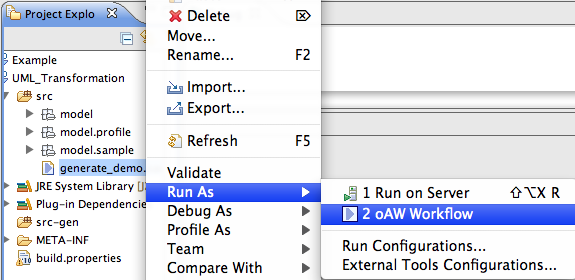
\includegraphics[width=0.3\textwidth]{Pictures/runTransformationUMLAs}
\caption{\label{fig:runTransformationUMLAs}Run UML transformation workflow} 
\end{floatingfigure}
To generate the YAKINDU state chart, right-click on
\textbf{generate\_demo.oaw} and select \textbf{Run As} $\rightarrow$
\textbf{MWE Workflow} (Compare Figure \ref{fig:runTransformationUMLAs}). The
output of the transformation is saved in the new folder src-gen and the status
of the run is available in the Console view of eclipse, which will be
automatically opened in the right corner at the bottom of the window.

The result is a *.statemachine file which can be found in the src-gen folder
within your project. The output folder, where your statemachines will be generated
and the UML2 model can be defined in the generatordemo.oaw. The next step,
which should follow, is to generate a diagram for your model. This is not
automatically done, but with a right-click on the statemachine file you can
initialize a diagram (see figure \ref{fig:initializeDiagram}). Because the
layout information are not stored inside UML2 you have to draft your diagram
by hand. \begin{figure}[ht]
\center
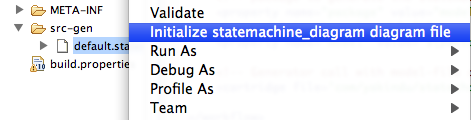
\includegraphics[width=0.6\textwidth]{Pictures/initializeDiagram}
\caption{\label{fig:initializeDiagram}Initialize Diagram} 
\end{figure}

The generated state chart can be edited, simulated and code can be generated
from it. These steps were described in previous chapters. If you want to
generate code from the state chart see Chapter \ref{sec:CCodeGenerator} for C
and Chapter \ref{sec:JavaCodeGenerator} for Java. If the model is a valid
YAKINDU state chart a simulation is also possible (see Chapter
\ref{sec:simulatingStateMachine}).

\section{How does it work}
The UML2 state machine and the YAKINDU state chart are quite similar.
Nevertheless, there are a few differences that need to be cared of.

\subsection{Name mapping}
The naming is the smallest gap. The following table shows the name mapping
between the UML2 state machine and the YAKINDU state chart.

\begin{table}[ht]
\begin{center}
\begin{tabular}{|c|c|}
\hline UML2 & YAKINDU \\
\hline
StateMachine & Statechart \\
Region & Region \\
Transition & Transition \\
Vertex & Node \\
State &  State \\
FinalState & FinalState \\
Pseudostate & Pseudostate \\
\hline
\end{tabular}
\end{center}
\caption{UML2 - YAKINDU Mapping}
\label{UML2 - YAKINDU Mapping}
\end{table}

As you can see, there are only marginal differences. Besides that, YAKINDU state
chart also defines new elements which are not present in the UML2.

\subsection{New elements}
The new elements are Variable and Event. As those can't be mapped 1:1, some
conventions are needed. The default behavior of the transformation is to ignore
those elements. This will result in an incomplete YAKINDU state chart (therefore
no simulation is possible). To %prevent this, you can decide between two methods.
prevent this, you have to extend your UML2 state machine.

\subsection{Limitations}
There are a few UML Elements that are currently not supported by the transformation. That includes the
PseudoStates
\begin{itemize}
\item join
\item fork
\item entryPoint
\item exitPoint
\item and terminate.
\end{itemize}
A transformation that encounters such
an element will fail.

\subsection{Transformation Cartridge}
The Transformation Cartridge allows you to integrate the YAKINDU Transformation into
your oAW Workflow. The cartridge expects the following parameters.

\begin{table}[ht]
\begin{center}
\begin{tabular}{|l|l|}
\hline Parameter & Description \\
\hline
umlModel & A path to your UML2 Model file. \\
srcgen &  The output folder where the generated *.statemachine files should be created. \\
package &  The root directory for the transformation. \\
\hline
\end{tabular}
\end{center}
\caption{YAKINDU Transformation Cartridge Parameters}
\label{YAKINDU Transformation Cartridge Parameters}
\end{table}

In your oAW Workflow it may look like this:\begin{verbatim}
...
<property name="umlModel" value="model/Simple.uml"/>
<property name="src-gen" value="src-gen"/>
<property name="config" value="src/" />

<!-- Generator call with model-file and output-folder -->
<cartridge file='com/yakindu/statechart/transformation/uml2/transform.oaw' 
	project="com.yakindu.statechart.transformation.examples.uml2"
 	umlModel="${umlModel}" 
 	src-gen="${src-gen}" 
 	config="${config}" />
...
\end{verbatim} 


\section{Extending an UML2 state machine}
% The first method is to modify your UML2 state machine.
Since there aren't UML2 Elements called Variable or Event, those have to be
created with the existing UML2 elements and the YAKINDU UML2 profile. The profile
allows you to give Transitions and Regions a priority and to describe Events as
Signals and Variables as Classes.

First you need to apply the YAKINDU UML2 profile.  Open your *.uml file and select the model.
Click on \textbf{UML Editor} $\rightarrow$ \textbf{Package} $\rightarrow$
\textbf{Apply Profile}. A new window pops up where you add the YAKINDU UML2
profile to your model. Press \textbf{Ok} and save the *.uml file. Now that the
profile has been loaded you need to apply the stereotypes to various elements.
You can do this with the UML Editor which has been used until now.
\begin{figure}[h!]
\center
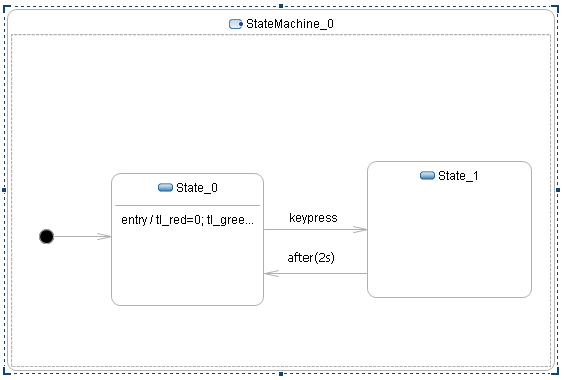
\includegraphics[width=0.5\textwidth]{Pictures/priorityVisualisation}
\caption{\label{fig:priorityVisualisation}UML2 state machine example} 
\end{figure}

Open the related *.umlstm file. It should look somehow like Figure
\ref{fig:priorityVisualisation}. The YAKINDU UML2 profile allows us to apply the
stereotypes Priority, Variable and Event. Priority can be applied to Transitions
and Regions, Variable to Classes and Event to Signals. First, we want to give
every Transition and every Region a Priority. To do so, select a
Transition/Region in the UML Editor. Select \textbf{UML Editor} $\rightarrow$ \textbf{Element} $\rightarrow$
\textbf{Apply Stereotype\dots}. Afterwards you can edit the priority in the properties tab, if element is selected.
\begin{figure}[h!] \center
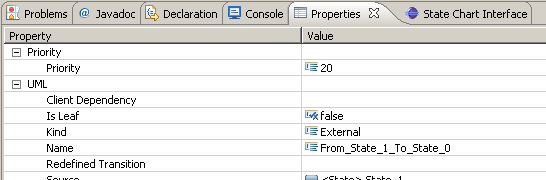
\includegraphics[width=0.9\textwidth]{Pictures/changePriority}
\caption{\label{fig:changePriority}Change the Priority} 
\end{figure}
The default value for Priority is 0 (see figure
\ref{fig:changePriority}). That's it! Repeat this for every Transition/Region in
your State machine.

Now we are going to add the Stereotypes Event to our Signals. Most work will be done in the tree UML Editor. 
\begin{figure}[h] \center
\includegraphics[width=0.9\textwidth]{Pictures/editorApplyStereotype}
\caption{\label{fig:editorApplyStereotype}Apply Stereotype} 
\end{figure}

Select a Signal and click on \textbf{UML Editor} $\rightarrow$ \textbf{Element}
$\rightarrow$\textbf{Apply Stereotype} (see figure
\ref{fig:editorApplyStereotype}). Add YAKINDU::Event and press \textbf{OK}. In
the Properties View you can see now a Property Event with some Attributes.
\begin{figure}[h] 
\center
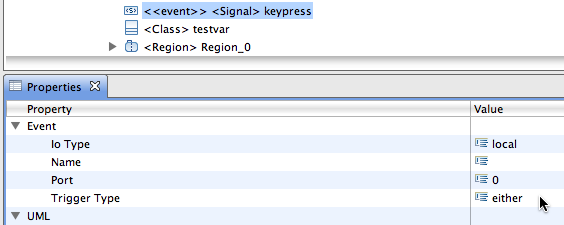
\includegraphics[width=0.9\textwidth]{Pictures/editorProperty}
\caption{\label{fig:editorProperty}Change Attributes} 
\end{figure}
Change those Attributes to your needs (see figure \ref{fig:editorProperty}).
Repeat this for every Signal in your state machine.

To add Variables to your UML2 state machine you have to create properties for your variable first. 
\begin{figure}[h] 
\center
\includegraphics[width=0.7\textwidth]{Pictures/variableExpression}
\caption{\label{fig:variableExpression}Property named after a Variable} 
\end{figure}

Those have to be named after the Variables in the Expressions of your Transitions
(see figure \ref{fig:variableExpression}). If you created a Property, select it and click
on \textbf{UML Editor} $\rightarrow$ \textbf{Element} $\rightarrow$
\textbf{Apply Stereotype}. Add YAKINDU::Variable and press \textbf{OK}. In the
Properties View you can change now the Attributes of Variable to your needs.
Repeat this for every Variable in you Expressions.

It is important to know that Signals and Properties that should be recognized as Events
and Variables must be created under the state machine in the UML2 model. This is
necessary due to the fact that any number of state machines can be in a UML2 model.

If you followed all the described steps you are now able to generate a valid
YAKINDU state chart.


%(ok)- how to use the transformation by example
%- how to simulate a transformed model
%(code?)- how to generate from a transformed model
%- how the transformation works (important mapping rules)
%-> Role of clasifier/class
%-> (done) using the profile
%-> (not yet) using alternatives to the profile


\clearpage
%%%%%%%%%%%%%%%%%%%%%%%%%%%%%%%%%%%%%%%%%%%%%%%%%%%%%%%%%%%%%%%%%%%%%%%%%%%
% Copyright (c) 2010 committers of YAKINDU and others.
% All rights reserved. This program and the accompanying materials
% are made available under the terms of the Eclipse Public License v1.0
% which accompanies this distribution, and is available at
% http://www.eclipse.org/legal/epl-v10.html
%
% Contributors:
%     committers of YAKINDU - initial API and implementation
%%%%%%%%%%%%%%%%%%%%%%%%%%%%%%%%%%%%%%%%%%%%%%%%%%%%%%%%%%%%%%%%%%%%%%%%%%%
\section{Example Scenario}

The example scenario is a simple pedestrian traffic light. A pedestrian can press
a button to indicate, she/he wants to cross the street. Then a blinking white
light indicates, that the traffic light has recognized the request. After a few
seconds, the traffic light for the street turns to red and the pedestrian traffic
light turns to green. Then the pedestrian traffic light turns to red and the
street traffic light changes to green again.
    
The state machine to model this behaviour is shown on figure
\ref{fig:statemachine}. This state machine must not be created but is shipped
with the example project and can be found in the
\texttt{workspace/Traffic\_Light/} directory.
    
\begin{figure}[ht] \center
\includegraphics[width=0.8\textwidth]{./Pictures/Statemachine}
\caption{\label{fig:statemachine}Statemachine for the Traffic Light Example}
\end{figure}

% The embedded system that is used with this scenario is a ATMega128 Controller
% on a Display3000 board. This system was extended by an additional board
% representing a traffic light controlled crossroad. This board is connected to
% the Display3000 board.

\section{Starting the workflow}

The source code is created by starting the MWE workflow. This workflow can be
found in the \textit{traffic light} example directory:

\begin{figure}[h!] \center
\includegraphics[width=0.8\textwidth]{./Pictures/workflow}
\caption{\label{fig:workflow}Starting the oAW-workflow to create the sources}
\end{figure}
\newpage

The generated C source code can be found within the new directory \texttt{c-src-gen}:

\begin{figure}[h!] \center
\includegraphics[width=0.3\textwidth]{./Pictures/sources}
\caption{\label{fig:sources}The sources are placed into the \textit{c-src-gen} directory}
\end{figure}

\newpage
%Hier fehlt noch was: wie wird der Workflow gestartet, und was muss alles vorhanden sein, damit der workflow tatsaechlich starten kann.
%-> Nutzer oAW
%-> Wo liegt das Ergebnis (Code)
%-> was kann man einstellen (Properties)

\section{Code Integration into an Existing Project}

Aside the source code for the state machine and the code for the interfaces, the
code generator creates a file called \texttt{make.include}. This file can easily
be included into an existing makefile by the line:

\begin{verbatim}
include c-src-gen/make.include
\end{verbatim}

The files, which are needed for the compilation, are added to the environment
variable \texttt{SM\_SOURCE}, so you have to add these sources to your project
sources:

\begin{verbatim}
OBJECTS    = main.o $(ENV_OBJ) $(GRAPHIC_OBJ) $(SM_SOURCE)
\end{verbatim}
%$

Additionally you should add the \texttt{c-src-gen} directory to the include and
source paths, so that the headers and sources could be found.
 
The example is designed for the Display3000 board, so the \textbf{Makefile} was
designed to create a binary for this hardware. Therefor it requires the AVR-gcc
toolchain to be able to compile. The toolchain contains a compiler, a linker and
some other usefull tools e.g. to download the data.

So go to your workspace directory with a shell and from there into the base
directory of your project and call \texttt{make}:

\begin{verbatim}
workspace$ cd Traffic_Light
Traffic_Light$ make
[...] compiling [...]
avr-gcc -Wall -Os -DF_CPU=7456000 -mmcu=atmega128 -I. -I./graphicLib [...]
rm -f main.hex
avr-objcopy -j .text -j .data -O ihex main.elf main.hex
\end{verbatim} 

If the compile was successful, you have a working binary \texttt{main.hex} that
could be deployed on the target.

To transfer the binary, you can use \texttt{make flash}.

\section{State Machine Access}

As mentioned before, the code for the state machine can be found in the folder
\textbf{c-src-gen}. After running the workflow the following files should be
available in this directory:

\begin{verbatim}
c-src-gen$ ls
make.include                        sm_trafficlightWaiting_PedWaiting.h
simElement.c                        trafficlightWaiting.c
simElement.h                        trafficlightWaiting.h
sm_trafficlightWaiting.c            trafficlightWaiting_Iface.c
sm_trafficlightWaiting.h            trafficlightWaiting_Iface.h
sm_trafficlightWaiting_Handle.c     trafficlightWaiting_timerIface.c
sm_trafficlightWaiting_Handle.h     trafficlightWaiting_timerIface.h
sm_trafficlightWaiting_PedWaiting.c
\end{verbatim}
% $

The files completely define the state machine. How to integrate the source into
another project, was subject of the previous section.

The files \texttt{sm\_trafficlightWaiting.*} and
\texttt{sm\_trafficlightWaiting\_PedWaiting.*} represents the two regions in the
state chart. The header- and C-file called
\texttt{sm\_trafficlightWaiting\_Handle.*} contain the main handle, which is
called \texttt{SM\_trafficlightWaiting\_Handle}. Please do not access the state
machine handle information directly.

The structure carries the information about the current state, the actual
transition, that has been activated, the handle for the first level region and
the interface handle. The handle is initialized with the function
\texttt{trafficlightWaiting\_init(\&sMachineHandle, \&interfaceHandle)}. Here the
\texttt{sMachineHandle} is the state machine handle and the
\texttt{interfaceHandle} is a \underline{pointer} to an interface handle. The
initialization call initializes the whole state machine and returns the interface
handle pointer.

For convenience all a state machine user needs to include is
\texttt{trafficlightWaiting.h}. This header includes all other necessary
information.
 
\section{Operating System and Drivers for the Example Device}

To let the state machine run on the Display 3000 development board, the system
needs a minimal \textbf{operating system} (OS) and some drivers for input and
output. This operating system is found in the \texttt{environment} directory.
This cooperative OS is written in C++ and contains an input driver for the 6 keys
on the hardware board and an output driver for the display and a LED board that
is connected to the \textit{port A}.

Because of copyright restrictions, the display driver is not included into this
example. The calls to the display interface can included by adding
\texttt{-DWITH\_DP3000\_GL} to the compiler options and updating the include
path defined in variable \texttt{COMPILETT} of the Makefile to point to the
right AVR-Libraries.

The transfer of the LED data uses a simple software driven SPI-like interface
with three connections (data, clock and inherit).

The rest, like shifting the data, is done by the hardware board.

Following files belong to the operating system:
\begin{verbatim}
definitions.h  event.h      scheduler.cpp  task.cpp
event.cpp      prioQueue.h  scheduler.h    task.h
\end{verbatim}

The \texttt{key*} files contain the driver for a debounced key input. The
\texttt{output*} files contain the driver code to create the output. To create
the cycles for the state machine, this behaviour is placed in the files
\texttt{statemachine*}.

\begin{figure}[h!]
\center
\includegraphics[width=0.8\textwidth]{./Pictures/Board1}
\caption{\label{fig:board1}Display3000 Development board with additional Hardware}
\end{figure}

After generation of source code by the workflow, it is possible to call the
Makefile inside the root directory of this example. By default this File calls
the commands \textbf{avr-gcc} and \textbf{avr-g++}. If you like to send
the binary to the micro controller, it is neccessary to check the \texttt{PORT}
variable inside the Makefile and \textbf{avrdude} needs to be on classpath. If
everything is correct, \texttt{make flash} will send the binary to the controller.
\newpage



%%%%% Java Generator Docs
\chapter{Java-Code Generator}
\label{sec:JavaCodeGenerator}
%%%%%%%%%%%%%%%%%%%%%%%%%%%%%%%%%%%%%%%%%%%%%%%%%%%%%%%%%%%%%%%%%%%%%%%%%%%
% Copyright (c) 2010 committers of YAKINDU and others.
% All rights reserved. This program and the accompanying materials
% are made available under the terms of the Eclipse Public License v1.0
% which accompanies this distribution, and is available at
% http://www.eclipse.org/legal/epl-v10.html
%
% Contributors:
%     committers of YAKINDU - initial API and implementation
%%%%%%%%%%%%%%%%%%%%%%%%%%%%%%%%%%%%%%%%%%%%%%%%%%%%%%%%%%%%%%%%%%%%%%%%%%%
\section{Introduction}
In our previous examples we created a YAKINDU state chart with the YAKINDU
Statechart Editor. However, it is also possible to import an existing UML2
state machine or create one with your favourite UML2 tool (You may also use
the UML2 Editor which ships with the eclipse modelling distribution). The tool
of your choice must support "EMF UML2". In our examples we are going to use
the UML2-Toools available in Galileo.

If you want to use an UML2 modelling tool instead of the YAKINDU Statechart
Editor or you have an existing UML2 state machine, you need to consider that
the YAKINDU state charts are somehow different from the UML2 state machines.
To fill this gap you have to extend your UML2 state machine (In future
releases another approach may also be available).

%or, if this is not anoption, you can create extensions for the transformation.

\section{UML2 model}
As for the code genenerators, an example project for transformation of UML2
state machines to YAKINDU state charts is also available. You can open the
examples (see Figure \ref{fig:uml2tools}) and compare them with the generated
YAKINDU state charts. \begin{figure}[ht]
\center
\includegraphics[width=1\textwidth]{Pictures/uml2tools}
\caption{\label{fig:uml2tools}UML2 state machine in eclipse} 
\end{figure}

Some information, which cannot be modelled in UML2 are generated
automatically, or as mentioned before, can be specified somehow else. For
example: Every Transition and every Region in a YAKINDU state chart needs a
priority. On how to set a priority will be discussed later. Lets have a look
at an example project first.

\section{The example project}
The example is available within eclipse under \textbf{File} $\rightarrow$
\textbf{New} $\rightarrow$ \textbf{Example\dots} within the category
\textbf{YAKINDU Examples}. Select ''UML -> YAKINDU Transformation'' and Finish the
dialog. A new project ''UML\_TransformationExample'' containing one UML
diagrams inclusive ''.umlstm'' diagram file for UML tools will be created.

\begin{floatingfigure}[r]{0.3\textwidth}
  \centering
\includegraphics[width=0.3\textwidth]{Pictures/runTransformationUMLAs}
\caption{\label{fig:runTransformationUMLAs}Run UML transformation workflow} 
\end{floatingfigure}
To generate the YAKINDU state chart, right-click on
\textbf{generate\_demo.oaw} and select \textbf{Run As} $\rightarrow$
\textbf{MWE Workflow} (Compare Figure \ref{fig:runTransformationUMLAs}). The
output of the transformation is saved in the new folder src-gen and the status
of the run is available in the Console view of eclipse, which will be
automatically opened in the right corner at the bottom of the window.

The result is a *.statemachine file which can be found in the src-gen folder
within your project. The output folder, where your statemachines will be generated
and the UML2 model can be defined in the generatordemo.oaw. The next step,
which should follow, is to generate a diagram for your model. This is not
automatically done, but with a right-click on the statemachine file you can
initialize a diagram (see figure \ref{fig:initializeDiagram}). Because the
layout information are not stored inside UML2 you have to draft your diagram
by hand. \begin{figure}[ht]
\center
\includegraphics[width=0.6\textwidth]{Pictures/initializeDiagram}
\caption{\label{fig:initializeDiagram}Initialize Diagram} 
\end{figure}

The generated state chart can be edited, simulated and code can be generated
from it. These steps were described in previous chapters. If you want to
generate code from the state chart see Chapter \ref{sec:CCodeGenerator} for C
and Chapter \ref{sec:JavaCodeGenerator} for Java. If the model is a valid
YAKINDU state chart a simulation is also possible (see Chapter
\ref{sec:simulatingStateMachine}).

\section{How does it work}
The UML2 state machine and the YAKINDU state chart are quite similar.
Nevertheless, there are a few differences that need to be cared of.

\subsection{Name mapping}
The naming is the smallest gap. The following table shows the name mapping
between the UML2 state machine and the YAKINDU state chart.

\begin{table}[ht]
\begin{center}
\begin{tabular}{|c|c|}
\hline UML2 & YAKINDU \\
\hline
StateMachine & Statechart \\
Region & Region \\
Transition & Transition \\
Vertex & Node \\
State &  State \\
FinalState & FinalState \\
Pseudostate & Pseudostate \\
\hline
\end{tabular}
\end{center}
\caption{UML2 - YAKINDU Mapping}
\label{UML2 - YAKINDU Mapping}
\end{table}

As you can see, there are only marginal differences. Besides that, YAKINDU state
chart also defines new elements which are not present in the UML2.

\subsection{New elements}
The new elements are Variable and Event. As those can't be mapped 1:1, some
conventions are needed. The default behavior of the transformation is to ignore
those elements. This will result in an incomplete YAKINDU state chart (therefore
no simulation is possible). To %prevent this, you can decide between two methods.
prevent this, you have to extend your UML2 state machine.

\subsection{Limitations}
There are a few UML Elements that are currently not supported by the transformation. That includes the
PseudoStates
\begin{itemize}
\item join
\item fork
\item entryPoint
\item exitPoint
\item and terminate.
\end{itemize}
A transformation that encounters such
an element will fail.

\subsection{Transformation Cartridge}
The Transformation Cartridge allows you to integrate the YAKINDU Transformation into
your oAW Workflow. The cartridge expects the following parameters.

\begin{table}[ht]
\begin{center}
\begin{tabular}{|l|l|}
\hline Parameter & Description \\
\hline
umlModel & A path to your UML2 Model file. \\
srcgen &  The output folder where the generated *.statemachine files should be created. \\
package &  The root directory for the transformation. \\
\hline
\end{tabular}
\end{center}
\caption{YAKINDU Transformation Cartridge Parameters}
\label{YAKINDU Transformation Cartridge Parameters}
\end{table}

In your oAW Workflow it may look like this:\begin{verbatim}
...
<property name="umlModel" value="model/Simple.uml"/>
<property name="src-gen" value="src-gen"/>
<property name="config" value="src/" />

<!-- Generator call with model-file and output-folder -->
<cartridge file='com/yakindu/statechart/transformation/uml2/transform.oaw' 
	project="com.yakindu.statechart.transformation.examples.uml2"
 	umlModel="${umlModel}" 
 	src-gen="${src-gen}" 
 	config="${config}" />
...
\end{verbatim} 


\section{Extending an UML2 state machine}
% The first method is to modify your UML2 state machine.
Since there aren't UML2 Elements called Variable or Event, those have to be
created with the existing UML2 elements and the YAKINDU UML2 profile. The profile
allows you to give Transitions and Regions a priority and to describe Events as
Signals and Variables as Classes.

First you need to apply the YAKINDU UML2 profile.  Open your *.uml file and select the model.
Click on \textbf{UML Editor} $\rightarrow$ \textbf{Package} $\rightarrow$
\textbf{Apply Profile}. A new window pops up where you add the YAKINDU UML2
profile to your model. Press \textbf{Ok} and save the *.uml file. Now that the
profile has been loaded you need to apply the stereotypes to various elements.
You can do this with the UML Editor which has been used until now.
\begin{figure}[h!]
\center
\includegraphics[width=0.5\textwidth]{Pictures/priorityVisualisation}
\caption{\label{fig:priorityVisualisation}UML2 state machine example} 
\end{figure}

Open the related *.umlstm file. It should look somehow like Figure
\ref{fig:priorityVisualisation}. The YAKINDU UML2 profile allows us to apply the
stereotypes Priority, Variable and Event. Priority can be applied to Transitions
and Regions, Variable to Classes and Event to Signals. First, we want to give
every Transition and every Region a Priority. To do so, select a
Transition/Region in the UML Editor. Select \textbf{UML Editor} $\rightarrow$ \textbf{Element} $\rightarrow$
\textbf{Apply Stereotype\dots}. Afterwards you can edit the priority in the properties tab, if element is selected.
\begin{figure}[h!] \center
\includegraphics[width=0.9\textwidth]{Pictures/changePriority}
\caption{\label{fig:changePriority}Change the Priority} 
\end{figure}
The default value for Priority is 0 (see figure
\ref{fig:changePriority}). That's it! Repeat this for every Transition/Region in
your State machine.

Now we are going to add the Stereotypes Event to our Signals. Most work will be done in the tree UML Editor. 
\begin{figure}[h] \center
\includegraphics[width=0.9\textwidth]{Pictures/editorApplyStereotype}
\caption{\label{fig:editorApplyStereotype}Apply Stereotype} 
\end{figure}

Select a Signal and click on \textbf{UML Editor} $\rightarrow$ \textbf{Element}
$\rightarrow$\textbf{Apply Stereotype} (see figure
\ref{fig:editorApplyStereotype}). Add YAKINDU::Event and press \textbf{OK}. In
the Properties View you can see now a Property Event with some Attributes.
\begin{figure}[h] 
\center
\includegraphics[width=0.9\textwidth]{Pictures/editorProperty}
\caption{\label{fig:editorProperty}Change Attributes} 
\end{figure}
Change those Attributes to your needs (see figure \ref{fig:editorProperty}).
Repeat this for every Signal in your state machine.

To add Variables to your UML2 state machine you have to create properties for your variable first. 
\begin{figure}[h] 
\center
\includegraphics[width=0.7\textwidth]{Pictures/variableExpression}
\caption{\label{fig:variableExpression}Property named after a Variable} 
\end{figure}

Those have to be named after the Variables in the Expressions of your Transitions
(see figure \ref{fig:variableExpression}). If you created a Property, select it and click
on \textbf{UML Editor} $\rightarrow$ \textbf{Element} $\rightarrow$
\textbf{Apply Stereotype}. Add YAKINDU::Variable and press \textbf{OK}. In the
Properties View you can change now the Attributes of Variable to your needs.
Repeat this for every Variable in you Expressions.

It is important to know that Signals and Properties that should be recognized as Events
and Variables must be created under the state machine in the UML2 model. This is
necessary due to the fact that any number of state machines can be in a UML2 model.

If you followed all the described steps you are now able to generate a valid
YAKINDU state chart.


%(ok)- how to use the transformation by example
%- how to simulate a transformed model
%(code?)- how to generate from a transformed model
%- how the transformation works (important mapping rules)
%-> Role of clasifier/class
%-> (done) using the profile
%-> (not yet) using alternatives to the profile


\clearpage
%%%%%%%%%%%%%%%%%%%%%%%%%%%%%%%%%%%%%%%%%%%%%%%%%%%%%%%%%%%%%%%%%%%%%%%%%%%
% Copyright (c) 2010 committers of YAKINDU and others.
% All rights reserved. This program and the accompanying materials
% are made available under the terms of the Eclipse Public License v1.0
% which accompanies this distribution, and is available at
% http://www.eclipse.org/legal/epl-v10.html
%
% Contributors:
%     committers of YAKINDU - initial API and implementation
%%%%%%%%%%%%%%%%%%%%%%%%%%%%%%%%%%%%%%%%%%%%%%%%%%%%%%%%%%%%%%%%%%%%%%%%%%%
\section{Setting Up The Example Project}

The reference example used within this documentation is the \emph{TrafficLight}
example project deployed with the YAKINDU distribution. To set it up in your
local workspace, use the YAKINDU Example Project Wizard as depicted by Figures
\ref{fig:screenshot1} and \ref{fig:screenshot2}. 
\begin{figure}[h!] 
\center
\includegraphics[width=0.5\textwidth]{./Pictures/Screenshot1}
\caption{\label{fig:screenshot1} Opening the Example Creation Wizard}
\end{figure}

\begin{figure}[h!]
\center
\includegraphics[width=0.5\textwidth]{./Pictures/Screenshot2}
\caption{\label{fig:screenshot2} Creating Statechart Example Projects}
\end{figure}

After successful completion, the Example Project Wizard will create the YAKINDU
Statechart example projects within the workspace, out of which one -
\emph{TrafficLight} - will serve as demonstration example in the following. As
outlined within Figure \ref{fig:screenshot3}, it denotes a state chart to control
a simple traffic light with a corresponding pedestrian light.

\begin{figure}[h!]
\center
\includegraphics[width=\textwidth]{./Pictures/Screenshot3}
\caption{\label{fig:screenshot3} Traffic Light Example Project Contents}
\end{figure}

\clearpage
%%%%%%%%%%%%%%%%%%%%%%%%%%%%%%%%%%%%%%%%%%%%%%%%%%%%%%%%%%%%%%%%%%%%%%%%%%%
% Copyright (c) 2010 committers of YAKINDU and others.
% All rights reserved. This program and the accompanying materials
% are made available under the terms of the Eclipse Public License v1.0
% which accompanies this distribution, and is available at
% http://www.eclipse.org/legal/epl-v10.html
%
% Contributors:
%     committers of YAKINDU - initial API and implementation
%%%%%%%%%%%%%%%%%%%%%%%%%%%%%%%%%%%%%%%%%%%%%%%%%%%%%%%%%%%%%%%%%%%%%%%%%%%
\section{Generating Source Code}

\subsection{Create Xtend Project}
The starting point to create Java source code from a YAKINDU Statechart model
is to set up a Java project to contain the generated code. For the sake of
simplicity, we will instead create a new Xtend project for this purpose (Xtend
projects also possess the Java as well as the PDE Plugin project nature), as
this allows to easily manage dependencies and execute MWE workflows. As
outlined by Figures \ref{fig:screenshot4}, \ref{fig:screenshot5}, and
\ref{fig:screenshot6}, creating an Xtend project is easily done using the
respective project creation wizard. Here, we choose \emph{TrafficLightJavaDemo}
as the name of the project.

\begin{figure}[h!]
\center
\includegraphics[width=0.5\textwidth]{./Pictures/Screenshot4}
\caption{\label{fig:screenshot4} Open New Wizard}
\end{figure}

\begin{figure}[h!]
\center
\includegraphics[width=0.5\textwidth]{./Pictures/Screenshot5}
\caption{\label{fig:screenshot5} Selecting to Create a new Xpand Project}
\end{figure}

\begin{figure}[h!]
\center
\includegraphics[width=0.5\textwidth]{./Pictures/Screenshot6}
\caption{\label{fig:screenshot6} Xtend Project Creation Wizard}
\end{figure}

%\begin{figure}[h!]
%\center
%\includegraphics[width=0.8\textwidth]{./Pictures/Screenshot7}
%\caption{\label{fig:screenshot7}}
%\end{figure}
\clearpage
\subsection{Manage Dependencies}
Having created the \emph{TrafficLightJavaDemo} project by means of the Xtend
project wizard, the next step is to make the YAKINDU Java code generator plugin
visible within the local project's classpath, so the Java code generation
cartridge file, which is deployed by the code generator plugin, can be
referenced from a local MWE workflow (to be set up as the next step). As we
have created a Xpand project (which is implicitly also a PDE plugin project, as
the Xpand project wizard adds the PDE plugin project nature to it), we may simply
do so by adding the YAKINDU Statchart Java code generator plugin to the list of
dependent plugins of our local project. As outlined by Figures
\ref{fig:screenshot8} and \ref{fig:screenshot9}, this can be simply achieved by
opening the manifest editor on the \texttt{MANIFEST.MF} file located within the
\texttt{META-INF} folder of the project, selecting the \texttt{Dependencies}
tab (depicted by Figure \ref{fig:screenshot8}, then by choosing to \emph{Add} a
new dependency and selecting the YAKINDU Statechart Java code generator
plugin in the resulting dialog (depicted Figure \ref{fig:screenshot9}).
Also the following Plug-Ins are required:
\begin{itemize}
\item org.eclipse.jface.text
\item org.eclipse.emf.mwe.utils
\item org.eclipse.emf.ecore.xmi
\item org.antlr.runtime
\item org.eclipse.xtext
\item org.eclipse.xtext.log4j
\item com.ibm.icu
\item org.eclipse.core.runtime
\item org.eclipse.jdt.core
\end{itemize}

\begin{figure}[h!]
\center
\includegraphics[width=\textwidth]{./Pictures/Screenshot8}
\caption{\label{fig:screenshot8} Manifest Editor}
\end{figure}

\begin{figure}[h!]
\center
\includegraphics[width=0.5\textwidth]{./Pictures/Screenshot9}
\caption{\label{fig:screenshot9} Adding Plugin Dependency}
\end{figure}

\clearpage
\subsection{Create MWE Workflow File}
As the YAKINDU Java code generator plugin provides an OAW workflow cartridge
that may most simply be called from within a local MWE workflow file, the next
step is to now set up such an MWE workflow file. This can be done as depicted
by Figures \ref{fig:screenshot10}, \ref{fig:screenshot11}, and
\ref{fig:screenshot12}, choosing \texttt{generate.wme} as the name of the
workflow file.

\begin{figure}[h!]
\center
\includegraphics[width=0.5\textwidth]{./Pictures/Screenshot10}
\caption{\label{fig:screenshot10} Opening New File Creation Wizard}
\end{figure}

\begin{figure}[h!]
\center
\includegraphics[width=0.5\textwidth]{./Pictures/Screenshot11}
\caption{\label{fig:screenshot11} Selecting to Create a new MWE Workflow File}
\end{figure}

\begin{figure}[h!]
\center
\includegraphics[width=0.5\textwidth]{./Pictures/Screenshot12}
\caption{\label{fig:screenshot12} Specifying Name of MWE Workflow File}
\end{figure}

\clearpage
The contents of the workflow file has to be added as outlined by
\ref{fig:screenshot13}. Basically, the location of the input YAKINDU
Statechart model (property \texttt{model}), as well as that of the output
folder (property \texttt{src-gen}), the Java source code has to be generated
into, have to be specified by means of workflow properties, being then passed
to the YAKINDU Statechart Java code generator cartridge
(\emph{generate\_java\_defensive.oaw}), which performs the actual code
generation.

\begin{figure}[h!]
\center
\includegraphics[width=\textwidth]{./Pictures/Screenshot13}
\caption{\label{fig:screenshot13}}
\end{figure}

In fact, the YAKINDU Statechart Java Codegenerator provides a lot of workflow
cartridges, namely \emph{generate\_java.oaw}, \emph{generate\_java\_me.oaw} and
\emph{generate\_java\_lejos.oaw}. Each has a defensive-version, which
basically generate the same sort of
Java source code, with the restriction that the \emph{defensive} version
generates additional defensive code, being used to check pre- and
post-conditions as well as invariants at runtime.
The Java-Codegenerator generates normal JavaSE-Code. The JavaME-Code is designed
for mobile devices, which doesn't supports all Javaclasses.
The third workflow cartridge generate Java-Code for leJOS, which can deploy on a
LEGO Mindstorm.

\clearpage
\subsection{Execute MWE Workflow}
Having specified all relevant workflow properties, and having specified to
call the code generator cartridge, the MWE workflow may then be simply
executed as depicted by Figure \ref{fig:screenshot14}. It will generate Java
source code into the selected folder (here, the local \texttt{src-gen} folder
within the \emph{TrafficLightJavaDemo} project).

\begin{figure}[h!]
\center
\includegraphics[width=0.5\textwidth]{./Pictures/Screenshot14}
\caption{\label{fig:screenshot14} Contents of MWE Workflow File}
\end{figure}

\clearpage
%%%%%%%%%%%%%%%%%%%%%%%%%%%%%%%%%%%%%%%%%%%%%%%%%%%%%%%%%%%%%%%%%%%%%%%%%%%
% Copyright (c) 2010 committers of YAKINDU and others.
% All rights reserved. This program and the accompanying materials
% are made available under the terms of the Eclipse Public License v1.0
% which accompanies this distribution, and is available at
% http://www.eclipse.org/legal/epl-v10.html
%
% Contributors:
%     committers of YAKINDU - initial API and implementation
%%%%%%%%%%%%%%%%%%%%%%%%%%%%%%%%%%%%%%%%%%%%%%%%%%%%%%%%%%%%%%%%%%%%%%%%%%%
\section{The Generated Source Code}

The Java source code generated by the YAKINDU Statechart Java code generator
consists of a set of generic classes (located within the
\texttt{com.yakindu.statechart} package) and a model specific state chart
implementation class, named according to the respective Statechart, here
\texttt{Traffic\-Light\-Statechart} within \texttt{trafficlight} package),
which is outlined by Figure \ref{fig:screenshot22}. It is the single class
that may be directly used by clients to integrate the generated code with
manually written or other generated code.

To obtain a new instance of the state chart implementation, the generated
implementation class offers a static method named \texttt{createInstance()}.
It returns a completely initialized state chart instance, which may be started
(via \texttt{enter()}), cyclically executed (via \texttt{runCycle()}), and
stopped again (via \texttt{leave()}).

Feeding the state chart with external events is done by passing respective
event constants (declared within the state chart implementation class) into
the state chart instance (via \texttt{setEvent()}) prior to executing a new
cycle (via \texttt{runCyle()}). Setting variable values is similarly possible
via respective selector methods generated into the implementation class (a
pair of getter and setter for each variable of the state chart). On each call
to \texttt{runCycle()}, the state chart reacts on all events currently raised
(since the completion of the prior cycle) and reads the variable values as
they are set when calling \texttt{runCycle()}. After \texttt{runCycle()} has
been completed, all events raised prior to its execution will be cleared and
the variables reflect the values as they result from the reaction of the state
chart.

\begin{figure}[h!]
\center
\includegraphics[width=\textwidth]{./Pictures/Screenshot22}
\caption{\label{fig:screenshot22}}
\end{figure}
\clearpage

%%%%%%%%%%%%%%%%%%%%%%%%%%%%%%%%%%%%%%%%%%%%%%%%%%%%%%%%%%%%%%%%%%%%%%%%%%%
% Copyright (c) 2010 committers of YAKINDU and others.
% All rights reserved. This program and the accompanying materials
% are made available under the terms of the Eclipse Public License v1.0
% which accompanies this distribution, and is available at
% http://www.eclipse.org/legal/epl-v10.html
%
% Contributors:
%     committers of YAKINDU - initial API and implementation
%%%%%%%%%%%%%%%%%%%%%%%%%%%%%%%%%%%%%%%%%%%%%%%%%%%%%%%%%%%%%%%%%%%%%%%%%%%
\section{Integrating Generated Java Code}

A demonstration example that reflects the integration of the Java code,
generated for the \emph{TrafficLight} example with manually written code is
deployed with the YAKINDU Statechart tools and may be created using the
example wizard as outlined by Figures \ref{fig:screenshot17} and
\ref{fig:screenshot18}.

\begin{figure}[h!]
\center
\includegraphics[width=0.45\textwidth]{./Pictures/Screenshot17}
\caption{\label{fig:screenshot17} Opening the Example Wizard}
\end{figure}


\begin{figure}[h!]
\center
\includegraphics[width=0.5\textwidth]{./Pictures/Screenshot18}
\caption{\label{fig:screenshot18} Creating a new Java Code Generator Example Project}
\end{figure}

\clearpage
As depicted by Figure \ref{fig:screenshot19} it contains some manually written
code (within the \texttt{src} folder) that realizes a Draw2d visualization of
a traffic light, being adapted (within the \texttt{CrossingDemo} main class)
to the generated source code of the \emph{TrafficLight} example (contained in
the \texttt{src-gen} folder of the example project).

\begin{figure}[h!]
\center
\includegraphics[width=\textwidth]{./Pictures/Screenshot19}
\caption{\label{fig:screenshot19} Traffic Light Java Demo Project Contents}
\end{figure}

\clearpage
As outlined in Figures \ref{fig:screenshot20} and \ref{fig:screenshot21}, the
\texttt{CrossingDemo} main class within the example project may be executed as
a Java application. It shows a visualization of the \emph{TrafficLight} state
chart variable values (by means of colors of the traffic and pedestrian lights
contained) and offers a button group, which prolongs respectively named events
to the \emph{TrafficLight} state chart.

\begin{figure}[h!]
\center
\includegraphics[width=0.45\textwidth]{./Pictures/Screenshot20}
\caption{\label{fig:screenshot20} Running CrossingDemo as Java Application}
\end{figure}

\begin{figure}[h!]
\center
\includegraphics[width=0.5\textwidth]{./Pictures/Screenshot21}
\caption{\label{fig:screenshot21} CrossingDemo Application}
\end{figure}

%%%%% UML Transformation
\chapter{UML Transformation}
\label{sec:UMLTransformation}
%%%%%%%%%%%%%%%%%%%%%%%%%%%%%%%%%%%%%%%%%%%%%%%%%%%%%%%%%%%%%%%%%%%%%%%%%%%
% Copyright (c) 2010 committers of YAKINDU and others.
% All rights reserved. This program and the accompanying materials
% are made available under the terms of the Eclipse Public License v1.0
% which accompanies this distribution, and is available at
% http://www.eclipse.org/legal/epl-v10.html
%
% Contributors:
%     committers of YAKINDU - initial API and implementation
%%%%%%%%%%%%%%%%%%%%%%%%%%%%%%%%%%%%%%%%%%%%%%%%%%%%%%%%%%%%%%%%%%%%%%%%%%%
\section{Introduction}
In our previous examples we created a YAKINDU state chart with the YAKINDU
Statechart Editor. However, it is also possible to import an existing UML2
state machine or create one with your favourite UML2 tool (You may also use
the UML2 Editor which ships with the eclipse modelling distribution). The tool
of your choice must support "EMF UML2". In our examples we are going to use
the UML2-Toools available in Galileo.

If you want to use an UML2 modelling tool instead of the YAKINDU Statechart
Editor or you have an existing UML2 state machine, you need to consider that
the YAKINDU state charts are somehow different from the UML2 state machines.
To fill this gap you have to extend your UML2 state machine (In future
releases another approach may also be available).

%or, if this is not anoption, you can create extensions for the transformation.

\section{UML2 model}
As for the code genenerators, an example project for transformation of UML2
state machines to YAKINDU state charts is also available. You can open the
examples (see Figure \ref{fig:uml2tools}) and compare them with the generated
YAKINDU state charts. \begin{figure}[ht]
\center
\includegraphics[width=1\textwidth]{Pictures/uml2tools}
\caption{\label{fig:uml2tools}UML2 state machine in eclipse} 
\end{figure}

Some information, which cannot be modelled in UML2 are generated
automatically, or as mentioned before, can be specified somehow else. For
example: Every Transition and every Region in a YAKINDU state chart needs a
priority. On how to set a priority will be discussed later. Lets have a look
at an example project first.

\section{The example project}
The example is available within eclipse under \textbf{File} $\rightarrow$
\textbf{New} $\rightarrow$ \textbf{Example\dots} within the category
\textbf{YAKINDU Examples}. Select ''UML -> YAKINDU Transformation'' and Finish the
dialog. A new project ''UML\_TransformationExample'' containing one UML
diagrams inclusive ''.umlstm'' diagram file for UML tools will be created.

\begin{floatingfigure}[r]{0.3\textwidth}
  \centering
\includegraphics[width=0.3\textwidth]{Pictures/runTransformationUMLAs}
\caption{\label{fig:runTransformationUMLAs}Run UML transformation workflow} 
\end{floatingfigure}
To generate the YAKINDU state chart, right-click on
\textbf{generate\_demo.oaw} and select \textbf{Run As} $\rightarrow$
\textbf{MWE Workflow} (Compare Figure \ref{fig:runTransformationUMLAs}). The
output of the transformation is saved in the new folder src-gen and the status
of the run is available in the Console view of eclipse, which will be
automatically opened in the right corner at the bottom of the window.

The result is a *.statemachine file which can be found in the src-gen folder
within your project. The output folder, where your statemachines will be generated
and the UML2 model can be defined in the generatordemo.oaw. The next step,
which should follow, is to generate a diagram for your model. This is not
automatically done, but with a right-click on the statemachine file you can
initialize a diagram (see figure \ref{fig:initializeDiagram}). Because the
layout information are not stored inside UML2 you have to draft your diagram
by hand. \begin{figure}[ht]
\center
\includegraphics[width=0.6\textwidth]{Pictures/initializeDiagram}
\caption{\label{fig:initializeDiagram}Initialize Diagram} 
\end{figure}

The generated state chart can be edited, simulated and code can be generated
from it. These steps were described in previous chapters. If you want to
generate code from the state chart see Chapter \ref{sec:CCodeGenerator} for C
and Chapter \ref{sec:JavaCodeGenerator} for Java. If the model is a valid
YAKINDU state chart a simulation is also possible (see Chapter
\ref{sec:simulatingStateMachine}).

\section{How does it work}
The UML2 state machine and the YAKINDU state chart are quite similar.
Nevertheless, there are a few differences that need to be cared of.

\subsection{Name mapping}
The naming is the smallest gap. The following table shows the name mapping
between the UML2 state machine and the YAKINDU state chart.

\begin{table}[ht]
\begin{center}
\begin{tabular}{|c|c|}
\hline UML2 & YAKINDU \\
\hline
StateMachine & Statechart \\
Region & Region \\
Transition & Transition \\
Vertex & Node \\
State &  State \\
FinalState & FinalState \\
Pseudostate & Pseudostate \\
\hline
\end{tabular}
\end{center}
\caption{UML2 - YAKINDU Mapping}
\label{UML2 - YAKINDU Mapping}
\end{table}

As you can see, there are only marginal differences. Besides that, YAKINDU state
chart also defines new elements which are not present in the UML2.

\subsection{New elements}
The new elements are Variable and Event. As those can't be mapped 1:1, some
conventions are needed. The default behavior of the transformation is to ignore
those elements. This will result in an incomplete YAKINDU state chart (therefore
no simulation is possible). To %prevent this, you can decide between two methods.
prevent this, you have to extend your UML2 state machine.

\subsection{Limitations}
There are a few UML Elements that are currently not supported by the transformation. That includes the
PseudoStates
\begin{itemize}
\item join
\item fork
\item entryPoint
\item exitPoint
\item and terminate.
\end{itemize}
A transformation that encounters such
an element will fail.

\subsection{Transformation Cartridge}
The Transformation Cartridge allows you to integrate the YAKINDU Transformation into
your oAW Workflow. The cartridge expects the following parameters.

\begin{table}[ht]
\begin{center}
\begin{tabular}{|l|l|}
\hline Parameter & Description \\
\hline
umlModel & A path to your UML2 Model file. \\
srcgen &  The output folder where the generated *.statemachine files should be created. \\
package &  The root directory for the transformation. \\
\hline
\end{tabular}
\end{center}
\caption{YAKINDU Transformation Cartridge Parameters}
\label{YAKINDU Transformation Cartridge Parameters}
\end{table}

In your oAW Workflow it may look like this:\begin{verbatim}
...
<property name="umlModel" value="model/Simple.uml"/>
<property name="src-gen" value="src-gen"/>
<property name="config" value="src/" />

<!-- Generator call with model-file and output-folder -->
<cartridge file='com/yakindu/statechart/transformation/uml2/transform.oaw' 
	project="com.yakindu.statechart.transformation.examples.uml2"
 	umlModel="${umlModel}" 
 	src-gen="${src-gen}" 
 	config="${config}" />
...
\end{verbatim} 


\section{Extending an UML2 state machine}
% The first method is to modify your UML2 state machine.
Since there aren't UML2 Elements called Variable or Event, those have to be
created with the existing UML2 elements and the YAKINDU UML2 profile. The profile
allows you to give Transitions and Regions a priority and to describe Events as
Signals and Variables as Classes.

First you need to apply the YAKINDU UML2 profile.  Open your *.uml file and select the model.
Click on \textbf{UML Editor} $\rightarrow$ \textbf{Package} $\rightarrow$
\textbf{Apply Profile}. A new window pops up where you add the YAKINDU UML2
profile to your model. Press \textbf{Ok} and save the *.uml file. Now that the
profile has been loaded you need to apply the stereotypes to various elements.
You can do this with the UML Editor which has been used until now.
\begin{figure}[h!]
\center
\includegraphics[width=0.5\textwidth]{Pictures/priorityVisualisation}
\caption{\label{fig:priorityVisualisation}UML2 state machine example} 
\end{figure}

Open the related *.umlstm file. It should look somehow like Figure
\ref{fig:priorityVisualisation}. The YAKINDU UML2 profile allows us to apply the
stereotypes Priority, Variable and Event. Priority can be applied to Transitions
and Regions, Variable to Classes and Event to Signals. First, we want to give
every Transition and every Region a Priority. To do so, select a
Transition/Region in the UML Editor. Select \textbf{UML Editor} $\rightarrow$ \textbf{Element} $\rightarrow$
\textbf{Apply Stereotype\dots}. Afterwards you can edit the priority in the properties tab, if element is selected.
\begin{figure}[h!] \center
\includegraphics[width=0.9\textwidth]{Pictures/changePriority}
\caption{\label{fig:changePriority}Change the Priority} 
\end{figure}
The default value for Priority is 0 (see figure
\ref{fig:changePriority}). That's it! Repeat this for every Transition/Region in
your State machine.

Now we are going to add the Stereotypes Event to our Signals. Most work will be done in the tree UML Editor. 
\begin{figure}[h] \center
\includegraphics[width=0.9\textwidth]{Pictures/editorApplyStereotype}
\caption{\label{fig:editorApplyStereotype}Apply Stereotype} 
\end{figure}

Select a Signal and click on \textbf{UML Editor} $\rightarrow$ \textbf{Element}
$\rightarrow$\textbf{Apply Stereotype} (see figure
\ref{fig:editorApplyStereotype}). Add YAKINDU::Event and press \textbf{OK}. In
the Properties View you can see now a Property Event with some Attributes.
\begin{figure}[h] 
\center
\includegraphics[width=0.9\textwidth]{Pictures/editorProperty}
\caption{\label{fig:editorProperty}Change Attributes} 
\end{figure}
Change those Attributes to your needs (see figure \ref{fig:editorProperty}).
Repeat this for every Signal in your state machine.

To add Variables to your UML2 state machine you have to create properties for your variable first. 
\begin{figure}[h] 
\center
\includegraphics[width=0.7\textwidth]{Pictures/variableExpression}
\caption{\label{fig:variableExpression}Property named after a Variable} 
\end{figure}

Those have to be named after the Variables in the Expressions of your Transitions
(see figure \ref{fig:variableExpression}). If you created a Property, select it and click
on \textbf{UML Editor} $\rightarrow$ \textbf{Element} $\rightarrow$
\textbf{Apply Stereotype}. Add YAKINDU::Variable and press \textbf{OK}. In the
Properties View you can change now the Attributes of Variable to your needs.
Repeat this for every Variable in you Expressions.

It is important to know that Signals and Properties that should be recognized as Events
and Variables must be created under the state machine in the UML2 model. This is
necessary due to the fact that any number of state machines can be in a UML2 model.

If you followed all the described steps you are now able to generate a valid
YAKINDU state chart.


%(ok)- how to use the transformation by example
%- how to simulate a transformed model
%(code?)- how to generate from a transformed model
%- how the transformation works (important mapping rules)
%-> Role of clasifier/class
%-> (done) using the profile
%-> (not yet) using alternatives to the profile


\clearpage

%%%%% Dynamic Systems (Damos)
\chapter{Dynamical Systems Modeler (DAMOS)}
\label{sec:Damos}
%%%%%%%%%%%%%%%%%%%%%%%%%%%%%%%%%%%%%%%%%%%%%%%%%%%%%%%%%%%%%%%%%%%%%%%%%%%
% Copyright (c) 2010 committers of YAKINDU and others.
% All rights reserved. This program and the accompanying materials
% are made available under the terms of the Eclipse Public License v1.0
% which accompanies this distribution, and is available at
% http://www.eclipse.org/legal/epl-v10.html
%
% Contributors:
%     committers of YAKINDU - initial API and implementation
%%%%%%%%%%%%%%%%%%%%%%%%%%%%%%%%%%%%%%%%%%%%%%%%%%%%%%%%%%%%%%%%%%%%%%%%%%%
In the field of engineering, technical systems are often described by the concept of a dynamical system, 
which is a mathematical formalization of a time-dependent process (e.g. swinging pendulum). The prevalent 
method for modeling dynamical systems is by using block diagrams, which specify the signal flow between 
the components of the system.

The Dynamical Systems Modeler (DAMOS) supports this modeling approach and consists of three components:
\begin {itemize}
\item a block diagram editor
\item a simulator
\item and code generator for efficient C code 
\end{itemize}

DAMOS itself is very modular and can be extended by custom block types and also the simulator and code generator can be customized. 

%\chapter{Editor Reference}
%%%%%%%%%%%%%%%%%%%%%%%%%%%%%%%%%%%%%%%%%%%%%%%%%%%%%%%%%%%%%%%%%%%%%%%%%%%%
% Copyright (c) 2010 committers of YAKINDU and others.
% All rights reserved. This program and the accompanying materials
% are made available under the terms of the Eclipse Public License v1.0
% which accompanies this distribution, and is available at
% http://www.eclipse.org/legal/epl-v10.html
%
% Contributors:
%     committers of YAKINDU - initial API and implementation
%%%%%%%%%%%%%%%%%%%%%%%%%%%%%%%%%%%%%%%%%%%%%%%%%%%%%%%%%%%%%%%%%%%%%%%%%%%
\section{Detailed usage information}

\subsection{Regions}
\label{sec:Regions}

A region is a sub-state machine that runs concurrently to the other regions. To
serialize the processing of the sub-state machines within the regions, the
regions possess a priority. The region with the highest priority is processed
first.

\begin{figure}[ht] \center
\includegraphics[width=0.7\textwidth]{./Pictures/RegionsPlain}
\caption{\label{fig:RegionsPlain}Three regions within a State Machine Diagram.}
\end{figure}

In the actual YAKINDU version, the regions are not hierarchically aggregatable.
  
\subsection{States}
\label{sec:States}

The states are the main elements of a state machine as they specify the possible
states the state machine consist of. Every state has a unique name, which must be
set by the user.

\begin{figure}[ht]
\center
\includegraphics[width=0.7\textwidth]{./Pictures/statesInRegions}
\caption{\label{fig:statesInRegions}Two regions with two states each}
\end{figure}

The parameters of this state are:

\begin{itemize}
\item \textbf{Entry:} The actions, which are performed on the arrival in this
state are specified in the $<entry>$ area. 
\item \textbf{Do:} The actions, which are performed while the state does not 
change, is specified in the $<do>$ area.
\item \textbf{Exit:} The actions, which are performed when a status is left, is
specified in the $<exit>$ area.
\end{itemize}

%Hier fehlt noch: wie genau ist die "expression" die hier einzutragen ist definiert.
 
\newpage 

\subsection{Pseudostates}
\label{sec:Pseudostates}

Pseudostates are states, that do not have any $<entry>$, $<do>$ or $<exit>$
areas. These states are used to specify special states like the \textbf{Initial
State} or the \textbf{Final State}.

Actually the following states are defined:

\begin{itemize}
\item \textbf{Initial State:} The \textbf{Initial State} is the state where the
state machine or the sub-state machine specified by a region start with. Usually
the \textbf{Initial State} is connected unconditionally with another normal
state. 
\item \textbf{Final State:} The \textbf{Final State} is the state where a
state machine ends. When the \textbf{Final State} is reached, the state machine
usually stops processing. 
\item \textbf{Shallow History:} The \textbf{Shallow
History} carries the last active state within a sub-state machine. When this
sub-state machine is re-entered, the last active state is set active again. 
\item \textbf{Deep History:} The \textbf{Deep History} works as the \textbf{Shallow
History} but can also handle nested sub-state machines, so that the correct
nested sub-state machine is used when a sub-state machine is entered. 
\item \textbf{Choice:} A \textbf{Choice} a an element to branch a transition. Every
branch of a transition must have it's own transition condition. An example is a
transition, that is started with a trigger signal and then splits up to arrive at
state X or state Y depending on a guard variable. 
\item \textbf{Junction:} The
\textbf{Junction} connects two transitions that have the same target state.
\end{itemize}

\subsection{Transitions}
\label{sec:Transitions}

\textbf{Transitions} specify the change from one state to another. Every
\textbf{Transition} must have a condition on which the state switch takes place.
The syntax for this condition is:

\begin{verbatim}
Trigger1, Trigger2, \dots, TriggerN[Guard]/Action1; Action2; \dots ActionM; 
\end{verbatim}

\begin{itemize}
\item \textbf{Trigger:} A trigger is activated by an outside event. If more than
one trigger is specified all triggers are connected by \textbf{OR}.

A special trigger is specified by the \textit{after($<duration>$)} keyword. This
keyword defines a duration after which a transition is performed. The
$<duration>$ is an integer number with a specifier (e.g. $after(12s)$).

\item \textbf{Guard:}  A guard is a boolean expression. Example: \texttt{A==B}
\item \textbf{Action:} An action consists of instructions, that should be
performed during transition. This action should be short to have a reliable flow.
\end{itemize}

Additionally every \textbf{Transition} needs a unique priority. The reason is
that every \textbf{Transition} have to be unique, so that the state machine
always behalves in the same way independent of the sequence the
\textbf{Transitions} are created for example.

\subsection{Variables and Events}

The state machine is driven only by triggers and guarded variables, as discussed
in section \ref{sec:Transitions}. These two types of variable data can only be
used within a transition expression, if the variables and events (which results
in triggers) are defined.

To define a variable or an event, you open the \textbf{State Chart Interface} and
right-click on either \textbf{Events} or \textbf{Variables}.

The dialog \textbf{Create Variable} requests at least a name for the variable.
Additionally, the variable can have a \textbf{Port}. The \textbf{I/O-type}
specifies whether the variable is a local, input or output variable. At last, the
\textbf{Data Type} can be chosen between integer (int), floating point (double)
or boolean (bool).

Events are very similar to variables. The main difference during event creation
is that you can not specify a \textbf{Data Type} but a \textbf{Trigger Type}
which can hold the values \textit{raising}, \textit{falling} or \textit{either}.

\subsection{Interfaces}

To interact with the state machine the system designer can add interface
functions within an actions expression. These functions must follow the
\textbf{Action Function Pointer} definition (i.e. the function is returning void
and does not have any parameter). To meet the MISRA requirements, a function
pointer must be a constant pointer, which means that the interface function must
be bound to the state machine during compile time. So there is no late binding
available in this case.


%%%%%%%%%%%%%%%%%%%%%%%%%%%%%%%%%%%%%%%%%%%%%%%%%%%%%%%%%%%%%%%%%%%%%%%%%%%%
% Copyright (c) 2010 committers of YAKINDU and others.
% All rights reserved. This program and the accompanying materials
% are made available under the terms of the Eclipse Public License v1.0
% which accompanies this distribution, and is available at
% http://www.eclipse.org/legal/epl-v10.html
%
% Contributors:
%     committers of YAKINDU - initial API and implementation
%%%%%%%%%%%%%%%%%%%%%%%%%%%%%%%%%%%%%%%%%%%%%%%%%%%%%%%%%%%%%%%%%%%%%%%%%%%
\section{Detailed usage information}

\subsection{Regions}
\label{sec:Regions}

A region is a sub-state machine that runs concurrently to the other regions. To
serialize the processing of the sub-state machines within the regions, the
regions possess a priority. The region with the highest priority is processed
first.

\begin{figure}[ht] \center
\includegraphics[width=0.7\textwidth]{./Pictures/RegionsPlain}
\caption{\label{fig:RegionsPlain}Three regions within a State Machine Diagram.}
\end{figure}

In the actual YAKINDU version, the regions are not hierarchically aggregatable.
  
\subsection{States}
\label{sec:States}

The states are the main elements of a state machine as they specify the possible
states the state machine consist of. Every state has a unique name, which must be
set by the user.

\begin{figure}[ht]
\center
\includegraphics[width=0.7\textwidth]{./Pictures/statesInRegions}
\caption{\label{fig:statesInRegions}Two regions with two states each}
\end{figure}

The parameters of this state are:

\begin{itemize}
\item \textbf{Entry:} The actions, which are performed on the arrival in this
state are specified in the $<entry>$ area. 
\item \textbf{Do:} The actions, which are performed while the state does not 
change, is specified in the $<do>$ area.
\item \textbf{Exit:} The actions, which are performed when a status is left, is
specified in the $<exit>$ area.
\end{itemize}

%Hier fehlt noch: wie genau ist die "expression" die hier einzutragen ist definiert.
 
\newpage 

\subsection{Pseudostates}
\label{sec:Pseudostates}

Pseudostates are states, that do not have any $<entry>$, $<do>$ or $<exit>$
areas. These states are used to specify special states like the \textbf{Initial
State} or the \textbf{Final State}.

Actually the following states are defined:

\begin{itemize}
\item \textbf{Initial State:} The \textbf{Initial State} is the state where the
state machine or the sub-state machine specified by a region start with. Usually
the \textbf{Initial State} is connected unconditionally with another normal
state. 
\item \textbf{Final State:} The \textbf{Final State} is the state where a
state machine ends. When the \textbf{Final State} is reached, the state machine
usually stops processing. 
\item \textbf{Shallow History:} The \textbf{Shallow
History} carries the last active state within a sub-state machine. When this
sub-state machine is re-entered, the last active state is set active again. 
\item \textbf{Deep History:} The \textbf{Deep History} works as the \textbf{Shallow
History} but can also handle nested sub-state machines, so that the correct
nested sub-state machine is used when a sub-state machine is entered. 
\item \textbf{Choice:} A \textbf{Choice} a an element to branch a transition. Every
branch of a transition must have it's own transition condition. An example is a
transition, that is started with a trigger signal and then splits up to arrive at
state X or state Y depending on a guard variable. 
\item \textbf{Junction:} The
\textbf{Junction} connects two transitions that have the same target state.
\end{itemize}

\subsection{Transitions}
\label{sec:Transitions}

\textbf{Transitions} specify the change from one state to another. Every
\textbf{Transition} must have a condition on which the state switch takes place.
The syntax for this condition is:

\begin{verbatim}
Trigger1, Trigger2, \dots, TriggerN[Guard]/Action1; Action2; \dots ActionM; 
\end{verbatim}

\begin{itemize}
\item \textbf{Trigger:} A trigger is activated by an outside event. If more than
one trigger is specified all triggers are connected by \textbf{OR}.

A special trigger is specified by the \textit{after($<duration>$)} keyword. This
keyword defines a duration after which a transition is performed. The
$<duration>$ is an integer number with a specifier (e.g. $after(12s)$).

\item \textbf{Guard:}  A guard is a boolean expression. Example: \texttt{A==B}
\item \textbf{Action:} An action consists of instructions, that should be
performed during transition. This action should be short to have a reliable flow.
\end{itemize}

Additionally every \textbf{Transition} needs a unique priority. The reason is
that every \textbf{Transition} have to be unique, so that the state machine
always behalves in the same way independent of the sequence the
\textbf{Transitions} are created for example.

\subsection{Variables and Events}

The state machine is driven only by triggers and guarded variables, as discussed
in section \ref{sec:Transitions}. These two types of variable data can only be
used within a transition expression, if the variables and events (which results
in triggers) are defined.

To define a variable or an event, you open the \textbf{State Chart Interface} and
right-click on either \textbf{Events} or \textbf{Variables}.

The dialog \textbf{Create Variable} requests at least a name for the variable.
Additionally, the variable can have a \textbf{Port}. The \textbf{I/O-type}
specifies whether the variable is a local, input or output variable. At last, the
\textbf{Data Type} can be chosen between integer (int), floating point (double)
or boolean (bool).

Events are very similar to variables. The main difference during event creation
is that you can not specify a \textbf{Data Type} but a \textbf{Trigger Type}
which can hold the values \textit{raising}, \textit{falling} or \textit{either}.

\subsection{Interfaces}

To interact with the state machine the system designer can add interface
functions within an actions expression. These functions must follow the
\textbf{Action Function Pointer} definition (i.e. the function is returning void
and does not have any parameter). To meet the MISRA requirements, a function
pointer must be a constant pointer, which means that the interface function must
be bound to the state machine during compile time. So there is no late binding
available in this case.


\end{document}
